\documentclass{article}[12pt]
\usepackage{physics}
\usepackage{setspace}
\usepackage{amsmath}
\usepackage{mathrsfs}
\usepackage{amssymb}
\usepackage{feynmp-auto}
\usepackage{tgtermes}
\usepackage{graphicx}
\usepackage{booktabs}
\usepackage{array}
\usepackage{caption}
\usepackage{listings}
\usepackage{xcolor}
\usepackage{helvet}
\definecolor{codegreen}{rgb}{0,0.6,0}
\definecolor{codegray}{rgb}{0.5,0.5,0.5}
\definecolor{codepurple}{rgb}{0.58,0,0.82}
\definecolor{backcolour}{rgb}{0.95,0.95,0.92}
\definecolor{lightgray}{rgb}{0.95,0.95,0.95}

\lstdefinestyle{mystyle}{
    backgroundcolor=\color{lightgray},   
    commentstyle=\color{codegreen},
    keywordstyle=\color{magenta},
    numberstyle=\tiny\color{codegray},
    stringstyle=\color{codepurple},
    basicstyle=\fontfamily{pcr}\selectfont\footnotesize,
    breakatwhitespace=false,         
    breaklines=true,                 
    captionpos=b,                    
    keepspaces=true,                 
    numbers=left,                    
    numbersep=5pt,                  
    showspaces=false,                
    showstringspaces=false,
    showtabs=false,                  
    tabsize=2
}

\lstset{style=mystyle}
\captionsetup{font=footnotesize}
\newcommand{\RN}[1]{%s
  \textup{\uppercase\expandafter{\romannumeral#1}}%
}
\usepackage{geometry}
\geometry{
 a4paper,
 left=25.4mm,
 right=25.4mm,
 top=30mm,
 bottom=25.4mm
 }
\begin{document}
\section*{1.Introduction}
\begin{spacing}{1.5}

The study of the correlation between the particle-like systems in a many-body framework can predict a wide range of novel phenomena in condensed matter physics, especially in the aspects of phase transition. 
This perspective is crucial for the recent advances in quantum technologies such as quantum simulators implemented through optical lattice, superconducting circuits, and quantum materials (e.g., quantum dots).

The Phase transition between metal and insulator is defined as a rapid transition of conductivity. In the metallic phase, inside the material structure, there are free electrons exist and make available to electric current flows throughout the material, in the insulating phase the electrons are bonded tightly with atoms which hinders the flow of electric current.Several theories have been developed to describe this phase transition phenomenon. In the Mott transition, the change of conductivity is explained through the Coulomb interactions between the electrons. While the density of the electrons inside the material becomes saturated, the interaction effect leads to repulsion between the particles which impedes current flow. Alternatively, In Andersen's transition model, the transition between the two phases is explained from more microscopic points of view by using the concept of disorder and impurities.

\subsection*{1.1  Summary}
In our study, we investigate the phase transition of a resistively shunted Josephson junction within the framework of the quantum impurity model. 
We establish a quantum mechanical framework based on the state vector of the macroscopic Josephson junction model. 
As starting in the very first step, we use impurity solving method (Non-crossing approximation, One-crossing approximation, TOA) in thermally stable state with Matsubara formalism , then evaluate the evolution of correlation of energy change ratio.

By employing the framework of strong correlation method, we expect a concrete description of the phase transition in a resistively shunted Josephson junction which is an ongoing debate. The precise nature of this transition is to be addressed through the analysis of the quantum state of electrons.
\begin{figure}[htbp]
  \centerline{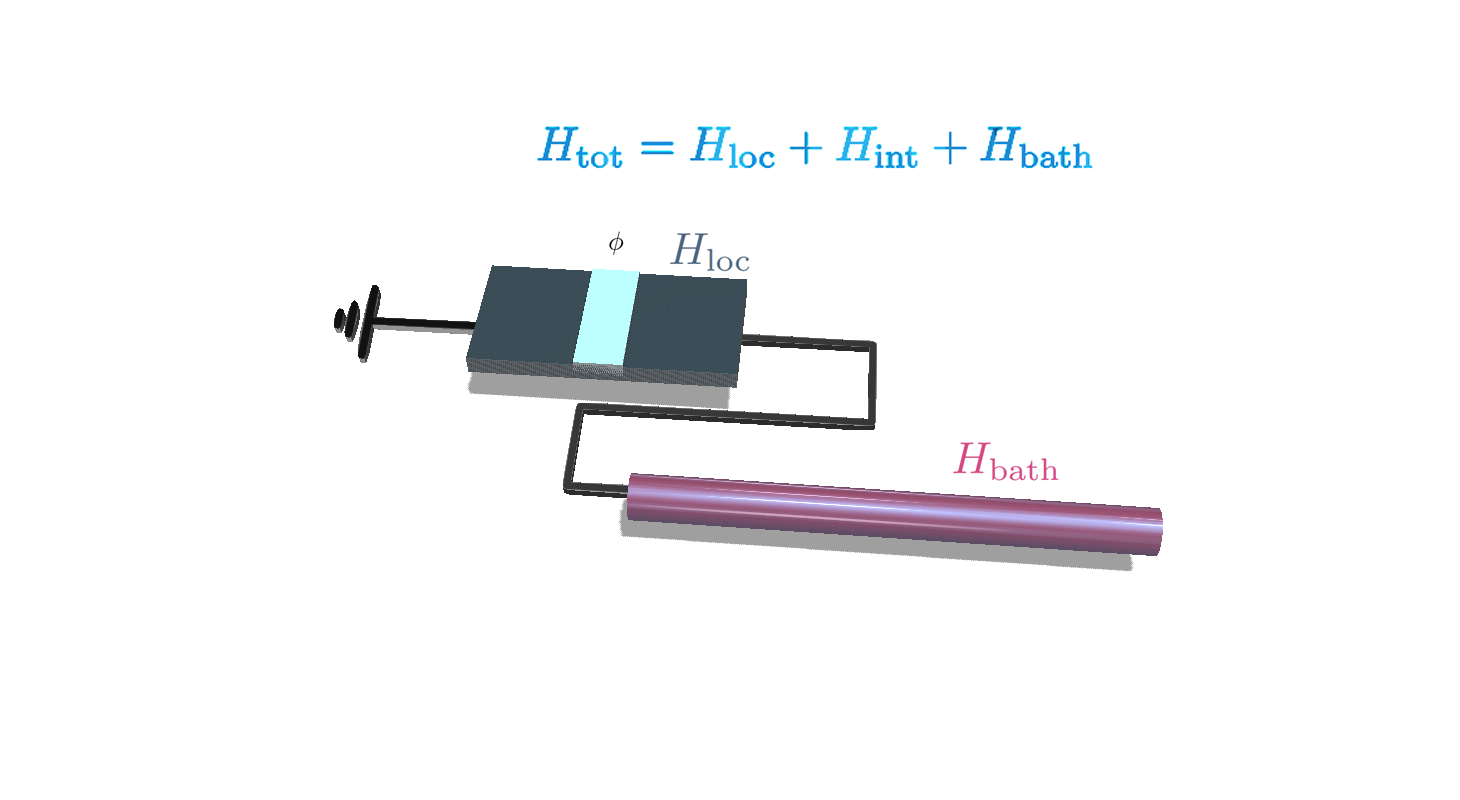
\includegraphics[width=10cm]{TexFigure/kps_create_junction.png}}
  \caption{Brief Image of total circuit.("LATER FIX")}
\end{figure}

\pagebreak
\subsection*{1.2  Previous work}

A resistively shunted Josephson junction(RSJJ) is a circuit consisting of a single Josephson junction simultaneously connected to an RC resonator structure which acts as a circuit resistance. Several studies have reported that the Josephson junction in this structure reveals a unique phase transition scheme that depends on the coupling strength between the Junction and the circuit resistance. This phenomenon allows RSJJ to play a physical role as a simulator for the quantum phase transition, especially for the Schmid quantum dissipative transition. Although RSJJ can be a well-defined physical structure for simulating the phase transition, it is limited to zero-temperature conditions, which is hard to achieve in an experimental approach.

\subsection*{1.3  Our approach}

\begin{figure}[htbp]
  \centerline{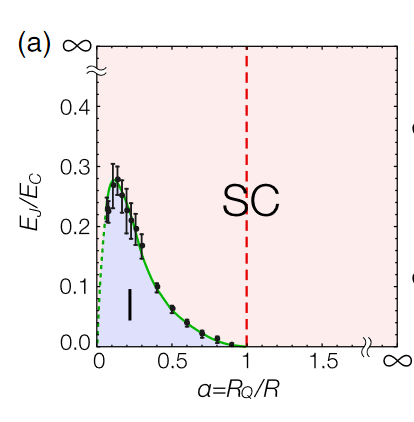
\includegraphics[width=7cm]{TexFigure/kps_INT_exp.PNG}}
  \caption{Zero temperature phase diagram with reentrant phase transition}
\end{figure}


In the latest study, a novel phase transition scheme called the ‘reentrant phase transition’ was predicted due to the potential independence of the dispersion relation of the RC resonator. Based on previous research, we’ll investigate this structure in a finite-temperature scheme. We construct the RSJJ Hamiltonian as a pseudo particle impurity model, which is described by the action of system $S$ separated into two parts: for local system $S_{loc}$ and for interaction $S_{int}$, 
\begin{flalign*}
S = S_{loc} + S_{int}  
\end{flalign*}

using Matsubara Green’s function. 

In our model, $S_{loc}$ will be correspond to the dynamics of Josephson junction, and $S_{int}$ will represents the interaction of Josephson junction and the RC resonator.

\end{spacing}

\pagebreak

\section*{2. Diagrammatic method}
\begin{spacing}{1.5}
In this chapter, We will briefly introduce the theoretical framework of the method of Green’s function, and pseudo-particle solvers, such as Non-crossing approximation. The detailed mathmatical derivation will treated on appendix.
\subsection*{2.1 Field operator and Green’s function}

In quantum many-body theory, the physical system is depicted over the frame of the fermionic(bosonic) creation and annihilation operator, and $\hat{a}(\hat{a}^\dagger)$ as an annihilation(creation) operator, it satisfies the following commutation relations:
\begin{flalign*}
[\hat{a_i},\hat{a_j}] &= \{\hat{a_i},\hat{a_j}\} = 0 \\ 
[\hat{a_i}^\dagger,\hat{a_j}^\dagger] &= \{\hat{a_i}^\dagger,\hat{a_j}^\dagger\}=0\\ 
[\hat{a_i},\hat{a_j}^\dagger] = \{\hat{a_i},\hat{a_j}^\dagger\} &= \delta_{ij} = \begin{cases} 1 \quad (i=j)\\  0 \quad (i \neq j)\quad \end{cases}
\end{flalign*}
Where the square bracket informs the bosonic case, and its RHS indicates the fermionic case. In the following discussion, we will drop out the lower indices of the field operator, assuming it can indicate any arbitrary quantum states.

If we consider the Hamiltonian system can be split into two parts: for the local system and for interaction, we can write the total Hamiltonian $H$:
\begin{flalign*}
H = H_0 + H_{int}
\end{flalign*}
Here, $H_0$ is the local(Free) Hamiltonian, $H_{int}$  is the Hamiltonian for interaction (external potential). To express the dynamics of a given operator, we depict the time dependency of the operator in the interaction picture :
\begin{flalign*}
\hat{a}(t) = e^{iH_0t}\hat{a}e^{-iH_0t} \\ \hat{a}^\dagger(t) =  e^{-iH_0t}\hat{a}^\dagger e^{iH_0t} 
\end{flalign*}
With the above time dependency, we can define the Green’s function as follows :
\begin{flalign*}
G_0(t,t') = \frac{i}{\hbar}\langle \mathcal{T}\hat{a}^\dagger(t)\hat{a}(t')\rangle = \begin{cases} \frac{i}{\hbar}\langle \hat{a}^\dagger(t)\hat{a}(t')\rangle  \quad (t>t')\\  \pm\frac{i}{\hbar}\langle \hat{a}(t')\hat{a}^\dagger(t)\rangle \quad (t<t')\quad \end{cases}
\end{flalign*}
Here, the symbol $\mathcal{T}$ is the time ordering operator. One of the features of Green’s function is that it satisfies the given equation of motion :
\begin{flalign*}
[i \partial_t-H] &G(t,t')=\delta(t-t') \\
[i \partial_t-H_0]G_0(t,t')&=[i \partial_t-H+H']G_0(t,t')=\delta(t-t')
\end{flalign*}
\subsection*{2.2 Diagrammatic expansion of Green’s function}

In the statistical framework, it is easy to calculate Green’s function in the imaginary time $\tau$ due to the wick rotation of the time axis, which mapped time-dependent system progression into thermal equilibrium problems with temperature dependency.
\begin{flalign*}
\frac{it}{\hbar}=\tau = \beta = \frac{1}{k_BT}
\end{flalign*}
We will use $\hbar=1$ in overall discussion. In this new frame, Green’s function can be rewritten :
\begin{flalign*}
G_0(\tau,\tau') = \langle\mathcal{T}\hat{a}^\dagger(\tau)\hat{a}(\tau)\rangle\begin{cases} \langle \hat{a}^\dagger(\tau)\hat{a}(\tau')\rangle  \quad (\tau>\tau')\\  \pm \langle \hat{a}(\tau')\hat{a}^\dagger(\tau)\rangle \quad (\tau<\tau')\quad \end{cases}
\end{flalign*}
There are particular relationship between real-time Green’s function and imaginary time(temperature dependence) Green’s function, which is :
\begin{flalign*}
G(t,t')\vert_{t=0} = \pm e^{\beta H} G(t,t')\vert_{t=i\beta}
\end{flalign*}

These temperature dependence Green’s function is often called in another term, Matsubara Green’s function. Single Green’s function corresponding with one specific imaginary time interval can be represented in a diagrammatic way, which is the very basic formulation of the diagrammatic method. We can draw a line from $\tau'$  to $\tau$,

\begin{minipage}{0.5\textwidth}
  \vfill
  \begin{fmffile}{MS_The_1}
    \begin{fmfgraph*}(120,80)
      \fmfleft{i1,i2}
      \fmfright{o1,o2}
      \fmf{fermion}{i1,v1,o1}
      \fmf{fermion}{i2,v2,o2}
      \fmf{photon,tension=0.4}{v1,v2}
      \fmfdot{v1,v2}
    \end{fmfgraph*}
  \end{fmffile}
  \vfill
\end{minipage}
\hfill
\begin{minipage}{0.5\textwidth}
  \vfill
  \begin{fmffile}{MS_The_2}
    \begin{fmfgraph*}(120,80)
      \fmfleft{i}
      \fmfright{o}
      \fmf{fermion,tension=0.4}{i,v1,v2,o}
      \fmf{photon,left,tension=0}{v1,v2,v1}
      \fmfdot{v1,v2}
    \end{fmfgraph*}
  \end{fmffile}
  \vfill
\end{minipage}
\\
According to statistical mechanics, the expectation value of the physical observable is characterized by the partition function that satisfies the given restricted energy condition in phase space. Based on these concepts, on the grand canonical ensemble, the statistical structure of counting Green’s function becomes :  
\begin{flalign*}
G_0(\tau,\tau') = \frac{\text{Tr}[e^{-\beta H_0} \hat{a}^\dagger(\tau)\hat{a}(\tau')]}{\text{Tr}[e^{-\beta H_0}]} =\frac{\text{Tr}[e^{-\beta H_0} e^{iH_0 \tau} \hat{a}^\dagger e^{-H_0 (\tau-\tau')}\hat{a}e^{-iH_0 \tau'}]}{\text{Tr}[e^{-\beta H_0}]}
\end{flalign*}
This is the very basic form of Green’s function in imaginary time corresponding to the diagram structure. Similar case with the creation and annihilation operator, the time dependency of external potential term Hamiltonian : 
\begin{flalign*}
H'(\tau) = e^{H_0\tau}He^{-H_0\tau}
\end{flalign*}
If we consider the effect of interaction, we can adopt full Green’s function includes the interaction operator $U(\tau)$,
\begin{flalign*}
G(\tau,\tau') = \frac{\text{Tr}[e^{-\beta H_0} U(\beta)\hat{a}^\dagger(\tau)\hat{a}(\tau')]}{\text{Tr}[e^{-\beta H_0}U(\beta)]} =\frac{\text{Tr}[e^{-\beta H} U(\tau) \hat{a}^\dagger U(\tau'-\tau)\hat{a}U(\tau')]}{\text{Tr}[e^{-\beta H}]} 
\end{flalign*}
where interaction operator is : 
\begin{flalign*}
U(\tau) = \mathcal{T}e^{-\int^\tau_0 d\tau' H_{int}(\tau')}
\end{flalign*}
In the imaginary time interval $[\tau,0]$ , full Green’s function in the expectation form can be represented , 
\begin{flalign*}
G(\tau,0) = \frac{\text{Tr}[e^{-\beta H_0} U(\beta)\hat{a}^\dagger(\tau)\hat{a}]}{\text{Tr}[e^{-\beta H_0}U(\beta)]} = \frac{\langle U(\beta)\hat{a}^\dagger(\tau)\hat{a}\rangle_0}{\langle U(\beta)\rangle_0}
\end{flalign*}
The under index 0 of angled bracket indicates its expectation value was calculated in $H_{loc}$ frame. If the interaction hamiltonian is in the form of multiplication of pair of annihilation-creation operator $\hat{a}^\dagger$ and $\hat{a}$ , we can adjust Wick’s theorem to expand the each of the expectation value in denominator and numerator into a multiplication of Green’s functions in each time interval. For example, if 
\begin{flalign*}
H_{int} =V_{ijkl}\hat{a}^\dagger_i\hat{a}^\dagger_j\hat{a}_k\hat{a}_l
\end{flalign*}
Here the term $V_{ijkl}$ is the scalar value (or function) that represents the interaction effect. then 
\begin{flalign*}
\langle U(\beta)\rangle_0 \sim 1-\frac{1}{2}V_{ijkl}\int^\beta_0d\tau_1\langle\mathcal{T}\hat{a}^\dagger_i(\tau_1)\hat{a}_j^\dagger(\tau_1)\hat{a}_k(\tau_1)\hat{a}_l(\tau_1)\rangle + ... \\=1 - \frac{1}{2}\int^\beta_0\langle\mathcal{T}\hat{a}^\dagger_i(\tau_1)\hat{a}_j^\dagger(\tau_1)\rangle \langle\mathcal{T}\hat{a}_k(\tau_1)\hat{a}_l(\tau_1)\rangle + ...
\end{flalign*}

This kind of form of expansion represents the expectation value of the interaction operator in the multiplication of diagrams.
\pagebreak

\subsection*{2.3 Diagrammatic Hybridization expansion in strong coupling case}
In this section, we will introduce the hybridization method based on the former discussion. We follow the notation of []. In the case of the impurity model with a bosonic bath, the action of the full system can be written into : 
\begin{flalign*}
S = \int^\beta_0 d\tau H_{loc}(\tau) + \int^\beta_0 d\tau d\tau' P(\tau)\mathcal{W}(\tau-\tau')P(\tau')
\end{flalign*}
Here, $H_{loc}$is the Hamiltonian of the local system, indicating the impurity that we want to focus on. The terms $P$ and $\mathcal{W}$ correspond with the Hermitian operator and the interaction term can be assumed as $\mathcal{W}$ in the previous section.  As we treat the interaction Hamiltonian in the previous section, the term $\mathcal{W}$ includes the scalar factor to represent the effect of the bosonic bath. 
With similar procedure with the diagram expansion, We can calculate the expectation value of observable using the partition function $Z$,
\begin{flalign*}
Z=\text{tr}\bigg[T_{\tau}e^{-S}\bigg]
\end{flalign*}
And in the given frame, the expectation value of observable $O$ can be measured as 
\begin{flalign*}
\langle T_\tau O(\tau)\rangle = \frac{\text{tr}[T_{\tau}e^{-S} O(\tau)]}{\text{tr[}T_{\tau}e^{-S}]}
\end{flalign*}
Which has a similiar form of the full Green’s function. Similiar with it’s diagrammatic expansion, the partition function can be expanded to 
\begin{flalign*}
Z=\sum^{\infty}_{n=0}Z^{(n)}
\end{flalign*}
With it’s full expression, 
\begin{flalign*}
Z=&\sum_{n=0}^\infty \frac{(-1)^n}{n!} \sum_{\pi \in S_{2n}}\int^\beta_0d\tau_1\int^{\tau_1}_0 d\tau_2 \cdots\int^{\tau_{2n-1}}_0 d\tau_{2n}\text{tr}\bigg[U(\beta-\tau_1)PU(\tau_1-\tau_2)P\cdots P U(\tau_{2n})\bigg] \\
&\times\mathcal{W}(\tau_{\pi(1)}-\tau_{\pi(2)})\cdots\mathcal{W}(\tau_{\pi(2n-1)}-\tau_{\pi(2n)})
\end{flalign*}
Here, $\pi(m)$  refers that there are permutations and $S_{2n}$ is a set of available permutations for time ordering. The main Idea of the expansion is, that we only consider the certain “partial set” of full permutation, which corresponds with the non-crossing or crossing connected diagrams. Define the new $\bar{\mathcal{W}}$ function, 
\begin{flalign*}
\bar{\mathcal{W}} = (\mathcal{W}(\tau) + \mathcal{W}(-\tau))
\end{flalign*}
And consider the permutation which only restricted on the case of ,
\begin{flalign*}
\pi(2j-1) < \pi(2j)
\end{flalign*}
We can consider the normalization of the partition function using the chemical potential $\lambda$ in a grand canonical ensemble. With the normalization and the above two rules, we can construct the new formula about the expansion of the partition function, which can be rewritten as :
\begin{flalign*}
\mathcal{G}(\tau) = \sum^{\infty}_{n=0} \mathcal{G}^{(n)}(\tau) = e^{\tau \lambda}Z
\end{flalign*}
which is : 
\begin{flalign*}
\mathcal{G}^{(0)}(\tau) &= \mathcal{G}_{0}(\tau) \\ \mathcal{G}^{(1)} (\tau) &= \int^\beta_0 d\tau_1 \int^{\tau_1}_0 d\tau_2 \bigg[  \mathcal{G}_{i}(\beta-\tau) P \mathcal{G}_{i}(\tau_1 - \tau_2) P\mathcal{G}_{i}(\tau_2)\bigg] \bar{\mathcal{W}}(\tau_1 - \tau_2)\\
\mathcal{G}^{(2)} (\tau) &= \int^\beta_0 d\tau_1 \int^{\tau_1}_0 d\tau_2 \int^{\tau_2}_0 d\tau_3 \int^{\tau_3}_0 d\tau_4 \bigg[  \mathcal{G}_{i}(\beta-\tau) P \mathcal{G}_{i}(\tau_1 - \tau_2)P \mathcal{G}_{i}(\tau_2 - \tau_3)P \mathcal{G}_{i}(\tau_3 - \tau_4) P\mathcal{G}_{i}(\tau_4)\bigg ]\\ &\times \bigg(\bar{\mathcal{W}}(\tau_1 - \tau_2) \bar{\mathcal{W}}(\tau_3 - \tau_4) +\bar{\mathcal{W}}(\tau_1 - \tau_4) \bar{\mathcal{W}}(\tau_2 - \tau_3) +\bar{\mathcal{W}}(\tau_1 - \tau_3) \bar{\mathcal{W}}(\tau_2 - \tau_4) \bigg)
\end{flalign*}
The term $\mathcal{G}_i(\tau)$  is a matrix correspond with $U(\tau)$. During the calculation and the diagrams earned from the previous procedure, We can collect the irreducible diagrams that cannot be separated into a number of single propagators. These diagrams are defined self-energy, described as follows : 
\begin{flalign*}
\Sigma(\tau) = \sum_{n=1}^{\infty}\Sigma^{(n)}(\tau)
\end{flalign*}
and,
\begin{flalign*}
\Sigma^{(1)}(\tau) &= \bigg[P\mathcal{G}_{i}(\tau)P\bigg]\bar{\mathcal{W}}(\tau) \\ \Sigma^{(2)}(\tau) &= \int^\beta_0d\tau_1\int^{\tau_1}_0d\tau_2 \bigg[P\mathcal{G}_{i}(\tau-\tau_1)P\mathcal{G}_{i}(\tau_1-\tau_2)P\mathcal{G}_{i}(\tau_2)P\bigg](\bar{\mathcal{W}(\tau)}\bar{\mathcal{W}}(\tau_1-\tau_2) + \bar{\mathcal{W}}(\tau-\tau_2)\bar{\mathcal{W}}(\tau_1))
\end{flalign*}
Adopting the self-energy in normalized Partition function, we can gain the equation :
\begin{flalign*}
\mathcal{G} =& \mathcal{G}_{0}(\tau) + \int^\beta_0d\tau_1\int^{\tau_1}_0d\tau_2\mathcal{G}_{i}(\beta-\tau_1)\Sigma(\tau_1-\tau_2)\mathcal{G}^{(2)}(\tau_2) \\ 
&+ \int^{\beta}_0d\tau_1\int^{\tau_1}_0d\tau_2\int^{\tau_2}_0d\tau_3\int^{\tau_3}_0d\tau_4 \mathcal{G}_{i}(\beta-\tau_1)\Sigma(\tau_1-\tau_2)\mathcal{G}_{i}(\tau_2-\tau_3)\Sigma(\tau_3-\tau_4)\mathcal{G}_{i} + ...
\end{flalign*}
This form of Dyson equation can be represented into diagram structure. If we define full $\mathcal{G}$ as :
\begin{flalign*}
\mathcal{G} = \langle\psi_a(\tau)\psi_b^\dagger(\tau')\rangle = \text{Tr}[e^{\beta H}\psi_a(\tau)\psi_b^\dagger(\tau')]
\end{flalign*}
Then the diagram of the Dyson equation turns out to Figure.3.
\begin{figure}[htbp]
  \centerline{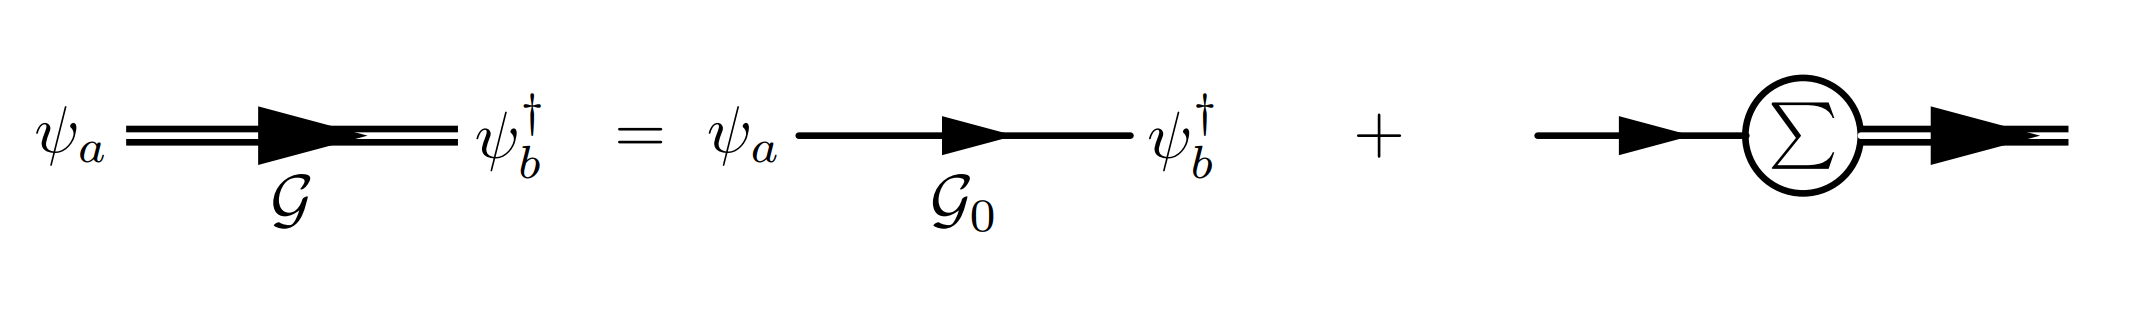
\includegraphics[width=13cm]{TexFigure/Dyson_eq.PNG}}
  \caption{Diagram for Dyson equation with self energy}
\end{figure}
While representing the self-energy in extended diagrammatic formation, we can collect the diagrams with some featured topological structures. For instance, if we consider only the first-order self-energy expansion, the result coincides with the well-known Non-crossing approximation method.
This form of equation satisfies the integral-differential form, agrees with the equation of motion of in the quantum mechanical aspect.
\begin{flalign*}
[-\partial_{\tau}-H_{loc}+\lambda]\mathcal{G}(\tau)-\int^\tau_0 d\tau_1\Sigma(\tau-\tau_1)\mathcal{G}(\tau_1) = 0 \quad, \quad(\tau>0)
\end{flalign*}
In our study, the function which corresponds with $\mathcal{W}$ is written as $V_k(\tau)$, 
\begin{flalign*}
V_k(\tau) = e^{-\omega_k\tau}\theta(-\tau)n_B(\omega_k \beta)  + e^{\omega_k\tau}\theta(\tau)(1+n_B(\omega_k \beta))
\end{flalign*}
Consider the form of $\bar{\mathcal{W}}$,
\begin{flalign*}
V_k(\tau)= e^{-\omega_k\tau} \frac{\cosh{\frac{\omega_k \beta}{2}}}{\sinh{\frac{\omega_k\beta}{2}}}
\end{flalign*}
\subsection*{Evaluation of correlation function}
We can get the connected diagram from the above procedures, and the connected correlation function can be calculated as:
\begin{flalign*}
c= \frac{\delta}{\delta a(\beta)}\frac{\delta}{\delta a(\tau)} \ln(Z[a(\tau)])\bigg\vert _{a=0}
\end{flalign*}
\end{spacing}
\pagebreak

\section*{3. Simulation model}
\begin{spacing}{1.5}
  \begin{figure}[htbp]
    \centerline{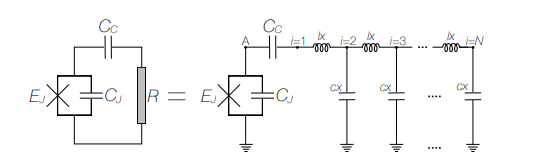
\includegraphics[width=12cm]{TexFigure/circuit_supp_ashida.PNG}}
    \caption{ Picture of resistivity shunted Josephson junction connected with exterior transmission line.}
  \end{figure}
  
We set the Resistivity shunted Josephson junction(RSJJ) circuit as an impurity model. 
Specific Hamiltonians and physical parameters used in the study are based on the paper. 
The circuit is composed of a single Josephson junction connected to the transmission line, 
which acts as the resistance of the total circuit system. 
Each component of the circuit is mapped onto each composition of the total Hamiltonian. 
The given circuit Hamiltonian form is represented as follows : 
\begin{flalign*}
H_{sys} = (E_c\hat{N^2}-E_J\cos{\phi})\otimes I -\hat{N}\otimes\sum_{0<k\leq K}\hbar g_k(\hat{b}_k^\dagger + \hat{b}_k) + I \otimes \sum_{0<k\leq K}\hbar\omega_k\hat{b_k}^\dagger\hat{b_k}
\end{flalign*}

Specific description of each parts of system Hamiltonian composed by : 
\begin{flalign*}
H_{loc} &=E_C\hat{N}^2 - E_J \cos{\phi} \\ H_{bath} &= \sum_{0<k\leq K} \hbar \omega_k \hat{b}^\dagger_k \hat{b}_k \\ H_{int} &= -\hat{N}\otimes\sum_{0<k\leq K} \hbar g_k (\hat{b}^\dagger_k + \hat{b}_k)
\end{flalign*}
The description of basic symbols is in Table. 1. Here the physical parameter [$\phi,\hat{N}]$ satisfies the commutation relation,
\begin{flalign*}
[\phi,\hat{N}]=i\hbar
\end{flalign*}
$\\$Interaction effect of local(impurity) system between bath is described through  
$g_k$ and the parameter $\alpha =\frac{R_Q}{R}$ .  We use $\alpha$ and $\gamma = \frac{E_J}{E_C}$ 
as parameters to control the criticality of the Josephson junction. We’ve set $E_C$ and $\hbar$ as energy units, 
1 as the value of each parameter during the calculation process. Detailed description of basic symbols is in Table. 1. 
\begin{table}[htbp]
  \centering
  \renewcommand{\arraystretch}{1.2}  % 행 간격 조정
  \begin{tabular}{@{}ccc@{}}
  \toprule
  \textbf{Symbols} & \textbf{Formula} & \textbf{Physical quantities} \\ 
  \midrule
  $\phi$ & & Phase of Josephson junction \\ 
  $\hat{N}$ & $-i\frac{\partial}{\partial \phi}$ & Charge operator \\ 
  $\omega_k$ & $vk =\frac{vm\pi}{L}$ & Bath frequency \\ 
  $\hat{b_k}^\dagger,\hat{b_k}$ & & Bosonic creation, annihilation operator \\
  $R_Q$ & $\frac{h}{4e^2}$ & Quantum resistance of junction \\
  $R$ & & Resistance of bath \\
  $E_C$ & $\frac{(2e)^2}{2C_J}$ & Josephson junction charging energy \\ 
  $E_J$ & & Josephson coupling energy \\ 
  $g_k$ & $\sqrt{\frac{2\pi v}{\alpha L} \frac{\omega_k}{1+(\frac{\nu \omega_k}{W})^2}}$ & Coupling with bath in mode $k$ \\ 
  $\nu$ & $\frac{\pi}{\alpha \epsilon_C}$ & \\
  $\epsilon_C$ & $\frac{E_C}{\hbar W}$ & \\
  \bottomrule
  \end{tabular}
  \caption{Table 1.Basic symbols used for describing Hamiltonian.}
  \end{table}


\subsection*{3.1 Span of $H_{loc}$ in Josephson effect basis}

To adjust the expansion method to the RSJJ Hamiltonian model, We represent the local system Hamiltonian in matrix formulation using the Josephson wave function as its basis. We adopt the macroscopic point of view to observe the superconducting effect expected in our junction system. The free-particle basis in exponential form is written as : 
\begin{flalign*}
\ket{\psi_{JJ}} = \sum_{-\infty}^{\infty} c_me^{im\phi}
\end{flalign*}

Here, $c_m$ and $m$ indicates the normalization factor and wave number which analogous to energy excitations. In trigonometric form, it turns out : 
\begin{flalign*}
\ket{\psi_{JJ}}=\sum_{m=0}^\infty a_m\cos{m\phi} +b_m\sin{m\phi}
\end{flalign*}

Where $a_m$ and $b_m$ are the normalization factor corresponds to even and odd trigonal function. separating in odd and even function,

\begin{flalign*}
\text{even part of the basis} : \sum_{m=0}^\infty a_m\cos{m\phi}\\\text{odd part of the basis} : \sum_{n=1}^\infty b_n\sin{n\phi}
\end{flalign*}

In a Hamiltonian of a system with arbitrary dimensions, the eigenvector written in the form of an even function in form of series expansion:
\begin{flalign*}
\ket{\text{even}_k}=\frac{a^{(k)}_0}{\sqrt{2\pi}} + \sum_{n=1}\frac{a^{(k)}}{\sqrt{\pi}}\cos{n\phi}
\end{flalign*}

Here, (k) represents the k-th split state, that is, the energy state of the even function basis split by external perturbation in the k-th excited state. In the same way, the eigenvector written in the form of an odd function is as follows: 
\begin{flalign*}
\ket{\text{odd}_k} = \sum_{m=1}\frac{b_m^{(k)}}{\sqrt{\pi}}\sin{m\phi}
\end{flalign*}

And its matrix form is : 
\begin{flalign*}
\ket{\text{even}_k}=\begin{pmatrix} \alpha_0 \\ \alpha_1\\ \vdots \\\alpha_m\end{pmatrix}\quad, \quad \ket{\text{odd}_k}=\begin{pmatrix} \beta_1 \\ \beta_2\\ \vdots \\\beta_m\end{pmatrix}
\end{flalign*}

We can span the target Hamiltonian in given basis.Considering the differential form of local system Hamiltonian with using above result,  
\begin{flalign*}
H_{loc} = -\frac{\partial^2}{\partial \phi^2} - \gamma\cos{\phi}
\end{flalign*}

\begin{flalign*}
&H_{loc}\ket{\psi_{JJ}} = H_{loc}(\ket{\text{even}_k}+\ket{\text{odd}_k}) \\ \text{ } \\ &\bigg(-\frac{\partial^2}{\partial \phi^2} - \gamma\cos{\phi}\bigg)\bigg(\sum_{m=0}^\infty a_m\cos{m\phi} +\sum_{n=1}^\infty b_n\sin{n\phi}\bigg) \\&= -\sum_{m=0}^\infty (ma_m\cos{m\phi}+\gamma\cos{\phi}\cos{m\phi})-\sum_{n=1}^\infty (nb_n\sin{n\phi}+\gamma\cos{\phi}\sin{n\phi})
\end{flalign*}

In matrix representation,
\begin{flalign*}
H_{\text{loc even}} = \begin{pmatrix}
\alpha_0 & -\frac{\gamma}{\sqrt{2}} & 0 & \cdots \\
-\frac{\gamma}{\sqrt{2}} & \alpha_1 & -\frac{\gamma}{2} & 0 & \cdots \\ &  \\
0 & -\frac{\gamma}{2} & \alpha_2 &  \\
\vdots &  &  & \ddots 
\end{pmatrix}
\end{flalign*}

\begin{flalign*}
H_{\text{loc odd}} = \begin{pmatrix}
\beta_1 & -\frac{\gamma}{2} & 0 & \cdots \\
-\frac{\gamma}{2} & \beta_2 & -\frac{\gamma}{2} & 0 & \cdots \\ &  \\
0 & -\frac{\gamma}{2} & \beta_3 &  \\
\vdots &  &  & \ddots 
\end{pmatrix}
\end{flalign*}

To study how system changes depends on coupling parameters and finite temperature conditions, we measure the total RSJJ Hamiltonian under local system basis engaged from diagonalization of the $H_{\text{loc even}}$ and $H_{\text{loc odd}}$ . 

\subsection*{3.2 Matrix form of $\hat{N}$  in local basis}

The charge operator $\hat{N}$ pursues polarization operator in our expansion model, endows coupling effect between local system and bath system. Exploiting local basis from previous procedure, We can write $\hat{N}$ in aspect of local system view.

\subsubsection*{2-level case}

Now, we can span the charge operator in eigenvectors of $H_{\text{loc even}}$ and $H_{\text{loc odd}}$. In 2-level case, we can use total lowest three states as basis vector,
\begin{flalign*}
&\ket{\text{gs}}=\frac{a^{(0)}_0}{\sqrt{2\pi}} + \sum_{n=1}\frac{a^{(0)}_n}{\sqrt{\pi}}\cos{n\phi} = \frac{a_0}{\sqrt{2\pi}} + \frac{a_1}{{\sqrt{\pi}}}\cos{\phi} + \frac{a_2}{\sqrt{\pi}} \cos{2\phi} +\cdots\\
&\ket{\text{1st}} = \sum_{m=1}\frac{b^{(1)}_m}{\sqrt{\pi}}\sin{m\phi} = \frac{b_1}{{\sqrt{\pi}}}\sin{\phi} +  \frac{b_2}{\sqrt{\pi}} \sin{2\phi}+\cdots\\
&\ket{\text{2nd}}=\frac{a^{(1)}_0}{\sqrt{2\pi}} + \sum_{n=1}\frac{a^{(1)}_n}{\sqrt{\pi}}\cos{n\phi}= \frac{a'_0}{\sqrt{2\pi}} + \frac{a'_1}{{\sqrt{\pi}}}\cos{\phi} + \frac{a'_2}{\sqrt{\pi}} \cos{2\phi} +\cdots
\end{flalign*}

Here we note the upper indices with round brace to indicate the energy excitation of local system. Then matrix form of $\hat{N}$ becomes :
\begin{flalign*}
\hat{N} &= \begin{pmatrix}
\bra{\text{gs}}-i\frac{\partial}{\partial\phi}\ket{\text{gs}} & \bra{\text{gs}}-i\frac{\partial}{\partial\phi}\ket{\text{1st}} & \bra{\text{gs}}-i\frac{\partial}{\partial\phi}\ket{\text{2nd}} \\
\bra{\text{1st}}-i\frac{\partial}{\partial\phi}\ket{\text{gs}} &  \bra{\text{1st}}-i\frac{\partial}{\partial\phi}\ket{\text{1st}} & \bra{\text{1st}}-i\frac{\partial}{\partial\phi}\ket{\text{2nd}} \\ 
\bra{\text{2nd}}-i\frac{\partial}{\partial\phi}\ket{\text{gs}} & \bra{\text{2nd}}-i\frac{\partial}{\partial\phi}\ket{\text{1st}} & \bra{\text{2nd}}-i\frac{\partial}{\partial\phi}\ket{\text{2nd}}
\end{pmatrix} \\ \quad \\ 
&=i\begin{pmatrix}
0 & \sum_{n=1}na^{(0)}_n b^{(1)}_n & 0\\
-\sum_{n=1}na^{(0)}_n b^{(1)}_n &  0 & -\sum_{n=1}na^{(1)}_n b^{(1)}_n \\ 
0 & \sum_{n=1}na^{(1)}_n b^{(1)}_n & 0
\end{pmatrix}
\end{flalign*}

\subsubsection*{Multilevel case}

For a 2-level system (without considering energy level splitting; the energy level needs to be split by external perturbation to become a 3-level Hamiltonian) or higher, the process of expressing the order parameter in matrix form for the Hamiltonian $H_{loc}$ of the system under consideration involves the following steps.
Now based on the above discussion, the extended form of charge operator in higher dimension is :
\begin{flalign*}
\hat{N} &= \begin{pmatrix}
\bra{\text{gs}}-i\frac{\partial}{\partial\phi}\ket{\text{gs}} & \bra{\text{gs}}-i\frac{\partial}{\partial\phi}\ket{\text{1st}} & \cdots \\
\bra{\text{1st}}-i\frac{\partial}{\partial\phi}\ket{\text{gs}} &  \ddots & \vdots \\ 
\vdots & \cdots & \bra{\text{nth}}-i\frac{\partial}{\partial\phi}\ket{\text{nth}}
\end{pmatrix} \\ \quad \\ 
&=i\begin{pmatrix}
0 & \sum_{n=1}na^{(0)}_n b^{(1)}_n & \cdots \\
-\sum_{n=1}na^{(0)}_n b^{(1)}_n &  \ddots & \ \\ & &-\sum_{n=1}na^{(n-1)}_n b^{(n)}_n \\ 
\vdots & \sum_{n=1}na^{(n-1)}_n b^{(n)}_n & 
\end{pmatrix}
\end{flalign*}
$\\$
In this case, the maximum dimension of $\hat{N}$  is $2n+1$ .

\subsection*{3.3 Transformation of the Order Parameter into Matrix Form}

The order parameter represents a set of values arranged in an ordered manner according to a specific rule for the system under consideration. In the investigation of phase transitions, we determine the current state of the system by observing changes in the order parameter.  In this simulation, the cosϕ function, which represents the phase difference of the Josephson current flowing on both sides of the Josephson junction, was set as the order parameter. A larger value of cosϕ can be interpreted as the phase difference of the currents flowing on both sides of the junction approaching 0. This indicates a state where current flows smoothly without the influence of resistance, suggesting that the entire junction is in a conductive state.

\subsubsection*{2-level case}

Since we aim to understand the system from the perspective of which represents the Josephson junction with three energy levels, 
we intend to expand order parameter $\cos \phi$ in simliar procedure with calculating $\hat{N}$ matrix. Adopting the form of fourier basis 
in the case of 2-level in the representing $\hat{N}$ matrix, cosϕ can be rewritten as a matrix operator, and 
\begin{flalign*}
\hat{\cos{\phi}} = \begin{pmatrix}
\bra{\text{gs}}\cos{\phi} \ket{\text{gs}} & \bra{\text{gs}}\cos{\phi}\ket{\text{1st}} & \bra{\text{gs}}\cos{\phi}\ket{\text{2nd}}  \\
\bra{\text{1st}}\cos{\phi}\ket{\text{gs}} & \bra{\text{1st}}\cos{\phi}\ket{\text{1st}} & \bra{\text{1st}}\cos{\phi}\ket{\text{2nd}}  \\
\bra{\text{2nd}}\cos{\phi}\ket{\text{gs}} & \bra{\text{2nd}}\cos{\phi}\ket{\text{1st}} & \bra{\text{2nd}}\cos{\phi}\ket{\text{2nd}} \\
\end{pmatrix} 
\end{flalign*}
When obtaining eigenvectors for the 2-level truncated 3*3 $H_{loc}$ matrix, the matrix form of $\cos\phi$ is expressed as follows.
\begin{flalign*}
\hat{\cos{\phi}} = \begin{pmatrix}
\frac{2}{\sqrt{2}}a_0a_1 + a_1a_2 & 0 & \frac{1}{\sqrt{2}}(a_1a'_0 + a_0a'_1) + \frac{1}{2}(a_1a'_2 + a_2a'_1)  \\
0 & b_1b_2 & 0  \\
\frac{1}{\sqrt{2}}(a_1a'_0 + a_0a'_1) + \frac{1}{2}(a_1a'_2 + a_2a'_1) & 0 & \frac{2}{\sqrt{2}}a'_0a'_1 + a'_1a'_2 \\
\end{pmatrix} 
\end{flalign*}
$\\$
\subsubsection*{Multilevel case}

For a 2-level system (without considering energy level splitting; the energy level needs to be split by external perturbation to become a 3-level Hamiltonian) or higher, the process of expressing the order parameter in matrix form for the Hamiltonian $H_{loc}$ of the system under consideration involves the following steps.
First, the calculation of the even function form of the order parameter $\cos \phi$ is as follows:
\begin{flalign*}
\cos{\phi} \ket{\text{even}_k} = \frac{a^{(k)}_0}{\sqrt{2\pi}}\cos{\phi} + \sum_{n=1}\frac{a^{(k)}}{\sqrt{\pi}}\cos{\phi}\cos{n\phi}
\end{flalign*}
And Final innerproduct result is:
\begin{flalign*}
\bra{\text{even}_l}\cos{\phi} \ket{\text{even}_k} = \int^{2\pi}_0\bigg(\frac{a^{(m)}_0}{\sqrt{2\pi}} + \sum_{m=1}\frac{a^{(m)}}{\sqrt{\pi}}\cos{m\phi}\bigg)\bigg(\frac{a^{(n)}_0}{\sqrt{2\pi}}\cos{\phi} + \sum_{n=1}\frac{a^{(n)}}{\sqrt{\pi}}\cos{\phi}\cos{n\phi}\bigg)
\end{flalign*}
The calculation for the odd function form is as follows:
\begin{flalign*}
\ket{\text{odd}}=\sum_{n=1} \frac{b_n^{(k)}}{\sqrt{\pi}}\sin{n\phi} \quad , \quad
\cos{\phi}\ket{\text{odd}}=\sum_{n=1}\frac{b_n^{(k)}}{\sqrt{\pi}}\cos{\phi}\sin{n\phi}
\end{flalign*}
Similar with the case of even state eigenvector, innerproduct result is:
\begin{flalign*}
    &\bra{\text{odd}_l}\cos{\phi} \ket{\text{odd}_k} = \sum_{n,m=1}\int^{2\pi}_0 d\phi \bigg(\frac{b_n^{(k)}b_m^{(l)}}{\pi}\cos{\phi}\sin{n\phi}\sin{m\phi}\bigg) \\
    &=    \left\{
        \begin{array}{ll}
            \text{if k} \nleq \text{l : }  \qquad \sum^N_{n=1} \bigg(\frac{\hat{b}^{(k)}_n\hat{b}^{(l)}_{n-1}}{2} + \frac{\hat{b}^{(k)}_n\hat{b}^{(l)}_{n+1}}{2}\bigg)\\
            \text{if k } \ngeq \text{l : }  \qquad \sum^N_{n=1} \bigg(\frac{\hat{b}^{(k)}_{n-1}\hat{b}^{(l)}_{n}}{2} + \frac{\hat{b}^{(k)}_{n+1}\hat{b}^{(l)}_{n}}{2}\bigg)
        \end{array}
        \right.
\end{flalign*}
Therefore, when the entire $\cos{\phi}$ is expressed in matrix form, it takes the following form:
\begin{flalign*}
    \hat{\cos{\phi}} = \begin{pmatrix}
       \ddots & & \vdots & & \\
      & \bra{\text{even}_k}\cos\phi\ket{\text{even}_k} & 0 & \bra{\text{even}_k}\cos\phi\ket{\text{even}_{k+1}} & \cdots \\
      & 0 & \bra{\text{odd}_k}\cos\phi\ket{\text{odd}_k} & 0 & \bra{\text{odd}_k}\cos\phi\ket{\text{odd}_{k+1}} \\
      & \bra{\text{even}_{k+1}}\cos\phi\ket{\text{even}_k} & 0 & \bra{\text{even}_{k+1}}\cos\phi\ket{\text{even}_{k+1}} & \\
      & & \vdots & &\ddots \\
      \end{pmatrix} 
    \end{flalign*}
And the expectation of order parameter can be calculated in following formula:
\begin{flalign*}
  \langle \cos\phi\rangle = \frac{\text{Tr}[\hat{\cos\phi}e^{\beta H}]}{\text{Tr}[e^{-\beta H}]}
\end{flalign*}
\end{spacing}
\pagebreak

\section*{4. Numerical Solution of the Integro-differential Equation}

\begin{spacing}{1.5}
The integro-differential equation central to the analysis of our model was solved numerically using C++ code.  This section outlines the key computational techniques employed within the code.

\subsection*{4.1 Structure of C++ code}
The structure of the C++ code designed to solve the integro-differential equation is outlined below. 
The C++ code for solving the integro-differential equation is structured as follows: the functions performing the calculations are declared beforehand within a header file (.hpp) using a class, and then defined within a source file (.cpp).
Appropriate numerical methods were adopted for each computational step.
$\\$
\begin{figure}[htbp]
  \centerline{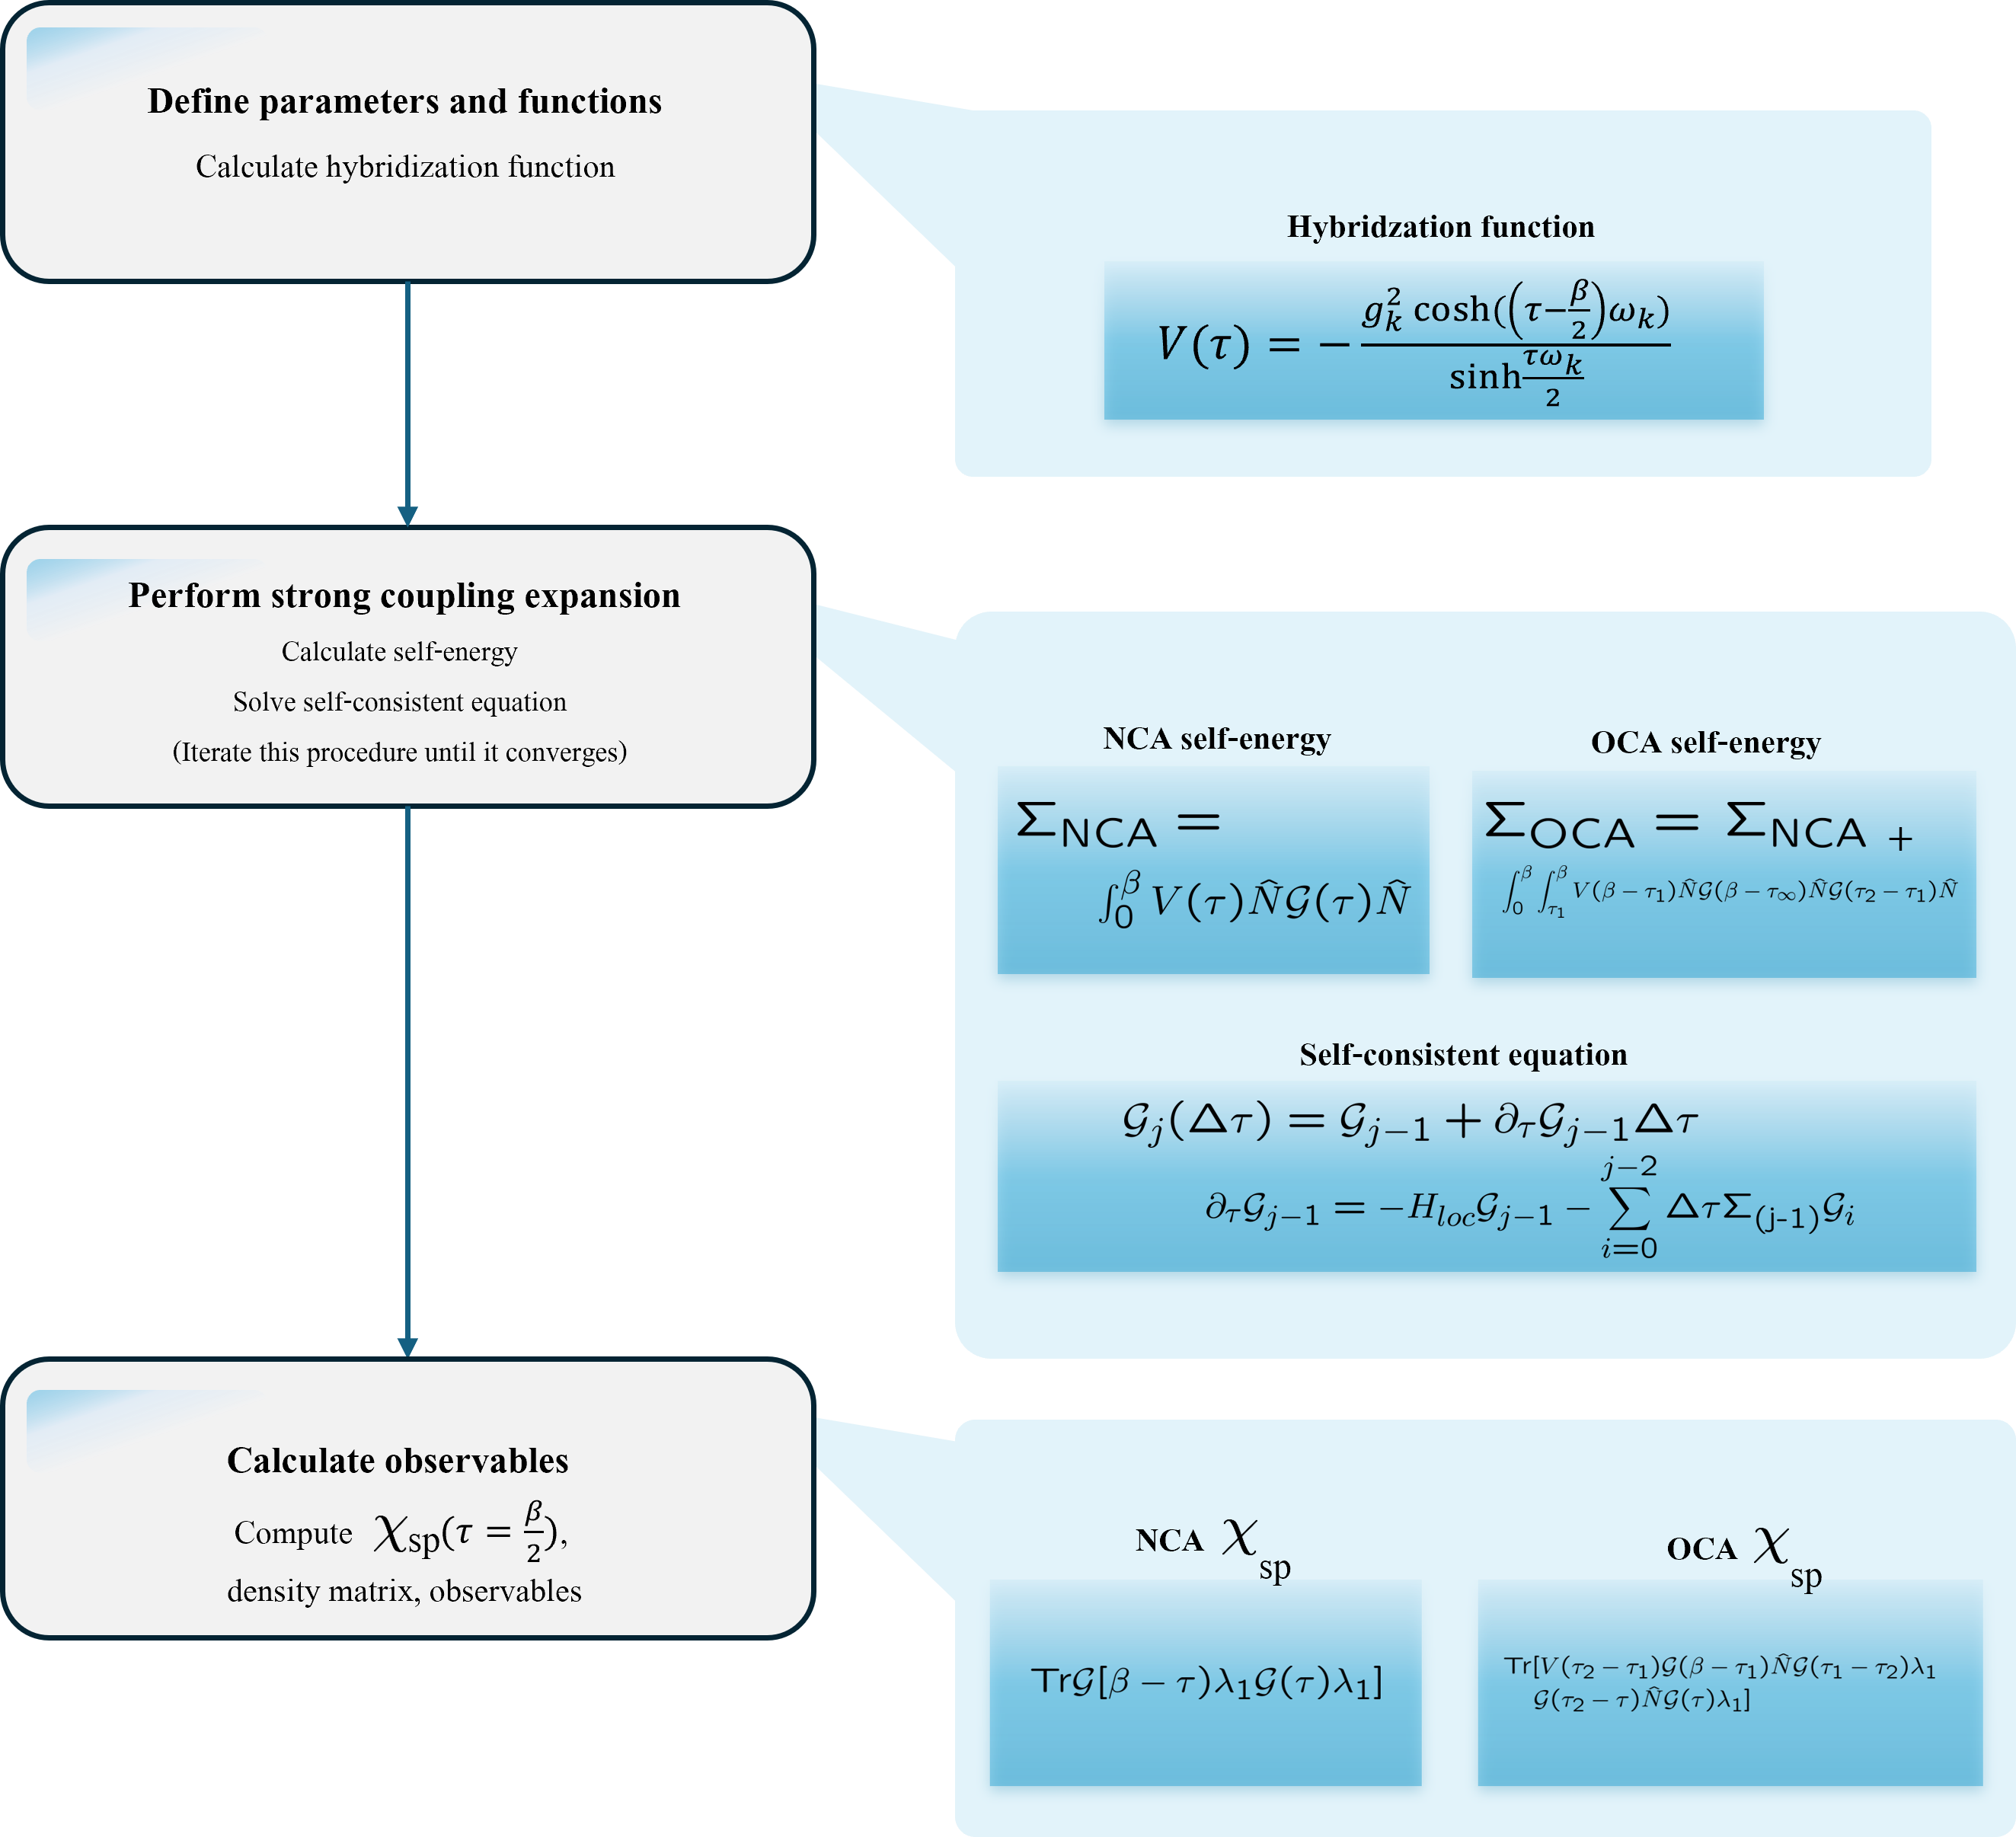
\includegraphics[width=13cm]{TexFigure/Flowchart_brokengraph.png}}
  \caption{The flowchart of Program structure}
\end{figure}

\subsection*{4.2 Hybridzation function - Simpson’s Rule}
The hybridization function, calculated as a scalar rather than a matrix, was evaluated by considering the form of the retarded Matsubara Green's function. To compute the value of $g_k$, a parameter that determines the coupling between the RC circuit and the Josephson junction, Simpson's rule of integration was employed. The formula for calculating $g_k$ for the application of this integration method is given below:
\begin{flalign*}
g_k =\sqrt{\frac{2W}{\alpha}\bigg(\frac{W}{1+(\nu x)^2}\bigg)} \qquad, \quad (x=\frac{k}{W})
\end{flalign*}
The integration method using Simpson’s method follows:
\begin{flalign*}
\int f(x) dx = \frac{b-a}{3n} \bigg[f(x_0) + \sum_{i=odd} 4f(x_i) + 2\sum_{i=\text{even}}f(x_i)+f(x_0) + f(x_f)\bigg]
\end{flalign*}
Here, we calculate the initial value using the case of $V(\tau,k=0)$. 
The part where the Simpson's rule is implemented in the code is as follows. After generating a vector array suitable for the length of the k-index to calculate  V(τ),  the integration is performed only for the k-value for $g_k$ and $\omega_k$ in the V(τ) expression. Using the resulting expression, the value for each τ interval is stored in an array of length τ.

\subsection*{4.3 Trapezoidal method}
The trapezoidal method was employed for the calculation of the self-energy and the propagator. This section provides a brief overview of the implementation for calculating the propagator. The numerical integration formula using the trapezoidal method is as follows: 

\begin{flalign*}
\int_{a}^{b} f(x) \, dx \approx \frac{\Delta x}{2} \left[ f(x_0) + 2f(x_1) + 2f(x_2) + \dots + 2f(x_{n-1}) + f(x_n) \right]
\end{flalign*}

To correspond to the actual numerical integration program code, the formula can be rewritten in the form of an infinite series as follows:
\begin{flalign*}
\int_{a}^{b} f(x) \, dx \approx \Delta x \left[ \frac{1}{2}f(x_0) + \sum_{j=1}^{n-1} f(x_j) +  \frac{1}{2}f(x_n) \right]
\end{flalign*}
And the self-consistent equation we aim to solve is as follows:
\begin{flalign*}
\mathcal{G}_j = \mathcal{G}_{j-1}+\partial_\tau\mathcal{G}_{j-1}\Delta\tau
\end{flalign*}
When implementing the trapezoidal method, it's crucial to follow a specific sequence of calculations:

1. First, update the value of $\partial_\tau\mathcal{G}_i$ using $\mathcal{G}_i$, which corresponds to each $f(x_i)$.

2. Next, calculate the temporary value of $\mathcal{G}'_{i+1}$ using the updated $\partial_\tau\mathcal{G}_i$.

3. Then, calculate $\partial_\tau\mathcal{G}_{i+1}$using the temporary value of $\mathcal{G}'_{i+1}$ calculated in the previous step.

4. Finally, perform the final trapezoidal integration calculation using $\frac{1}{2}(\partial_\tau\mathcal{G}_i + \partial_\tau\mathcal{G}_{i+1})$.
$\\$To implement this in the program, we introduced two arrays: P-array to store the final calculation result $\mathcal{G}_i$, 
and S-array to store the temporary value calculated in step 2. We also devised a method to use the value of S-array in step 3.
This process is visually represented in the diagram below, where:
\begin{figure}[htbp]
  \centerline{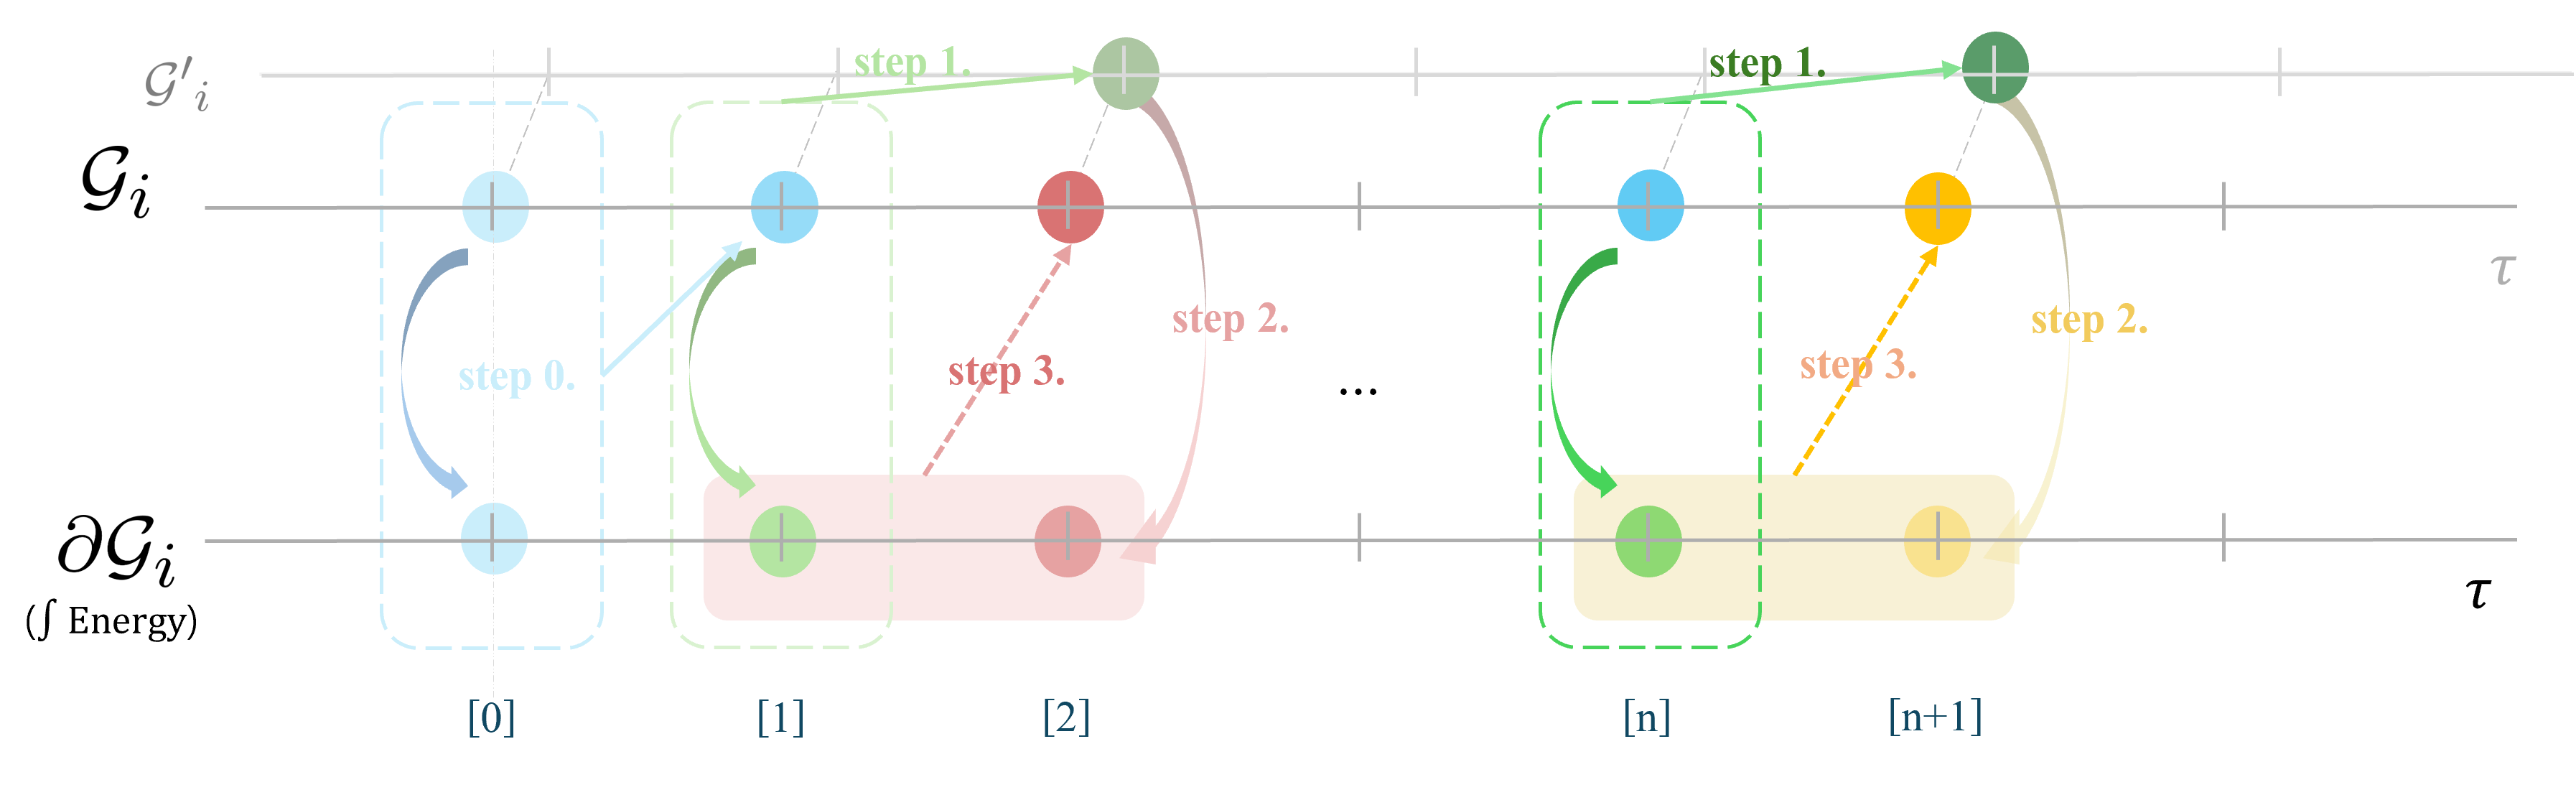
\includegraphics[width=15cm]{TexFigure/self_structure.png}}
  \caption{Image depicting the procedure of Trapezoidal process}
\end{figure}

This is implemented in the code as follows:
\begin{lstlisting}[language=C++, caption=Trapezoidal calculation code]
vector<MatrixXd> MD_OC::Propagator(const vector<MatrixXd>& sig, const MatrixXd& loc)
{
    vector<MatrixXd> P_arr(t, MatrixXd::Zero(siz,siz)); // Declaration of an array to store the final calculation result
    vector<MatrixXd> S_arr(t, MatrixXd::Zero(siz,siz)); // Declaration of an array to store temporary results during calculation
		
    P_arr[0] = MatrixXd::Identity(siz,siz);
    S_arr[0] = MatrixXd::Identity(siz,siz);

    MatrixXd sig_form = MatrixXd::Zero(siz,siz); // A matrix to temporarily store the result of process 1.
    MatrixXd sig_late = MatrixXd::Zero(siz,siz); // A matrix to temporarily store the result of process 3.


    for (int i = 1; i < t; i++)
    {
        P_arr[1] = P_arr[0];
        sig_late = 0.5 * Delta_t * (0.5 * Delta_t * (sig[1] * P_arr[0] + sig[0] * (P_arr[0] + Delta_t * P_arr[0])));
        P_arr[1] = P_arr[0] - 0.5 * Delta_t * loc * (2 * P_arr[0] + Delta_t * P_arr[0]) + sig_late;
        S_arr[1] = P_arr[1];

        if (i > 1)
        {
            sig_form = round_propagator_ite(loc, sig, P_arr, i - 1, 0);
            S_arr[i] = P_arr[i - 1] + Delta_t * sig_form; // Calculation process of 2. is performed in this part.

            sig_late = 0.5 * Delta_t * (round_propagator_ite(loc, sig, P_arr, i - 1, 1) + round_propagator_ite(loc, sig, S_arr, i, 1)); // This part is the result of performing trapezoidal calculation for the integral calculation in the round propagator.
            P_arr[i] = P_arr[i - 1] - 0.5 * Delta_t * loc * (2 * P_arr[i - 1] + Delta_t * sig_form) + sig_late; // This part is the result of performing trapezoidal calculation for the integral calculation in the round propagator.

        }
    }

    return P_arr;
}
\end{lstlisting}
\subsection*{4.4 Iteration truncation - Relative entropy}

The integro-differential equation we target to solve has a recursive structure, which means that a single calculation is not enough to get a complete result. The obtained array of $G(\tau)$ in the previous iteration is to be used as an initial condition for multiple iterative calculations until the result converges sufficiently. To truncate the iteration of calculations in flexibility, the concept of relative entropy was introduced into the code. The formula for calculating relative entropy is as follows:
\begin{equation*}
D(p||q) = \sum_{x\in\mathcal{X}}p(x)\ln\frac{p(x)}{q(x)}
\end{equation*}
In the case of $\mathcal{G}(\tau = \beta)$ in the interval $[0,\beta]$, The Green's function is represented by the same formula as the partition function of a thermal equilibrium state in the grand canonical ensemble. In this case, the partition function plays the same role as the density operator, which represents the mixed state of the system being investigated from a quantum mechanical perspective.
In quantum mechanics, each diagonal element of the density operator represents the probability of observing the corresponding energy level in the system. This allows us to calculate the probability distribution in the final stage. The code was designed to terminate the calculation of G(τ) when the distance between the probability distributions obtained at each calculation step becomes sufficiently small, indicating that the result has converged.

\begin{lstlisting}[language=C++, caption=Iteration truncation code]
// Function that returns the value of \mathcal{G}(\tau=\beta)
vector<double> MD_OC::temp_itemin(vector<MatrixXd> &arrr, double minpo, int size)
{
    vector<double> dist_return(size,0);
    for (int i = 0 ; i < size; i++){
        dist_return[i] = arrr[t-1](i,i); // Value of \mathcal{G} at \tau = \beta
    }
    return dist_return;
}

// Function that processes recursive calculation.
vector<MatrixXd> MD_OC::Iteration(const int& n)
{
    // ~ Calculation part
    //////////////////////////////////////////////////////////////
    double temp_minpoin;
    vector<vector<double> > temp_itemi(2,vector<double>(siz,0)); // Arrays to store the results of the previous and current iteration. siz represents the dimension of the calculated square matrix.
    double RELA_ENTROPY;
    ///////////////////////////////////////////////////////////////
    
    for (int i = 0; i <= n; i++){
        // ~ Calculation part
            //////////////////////////////////////////////////////////////////////////////

            temp_minpoin = //beta value; 

            //////////////////////////////////////////////////////////////////////////////
       // ~ Calculation part
           /////////////////////////////////////////////////////////////////////////////

            temp_itemi[(i-1)%2] = temp_itemin(Prop,temp_minpoin,siz); // temporary store previous iteration data
            RELA_ENTROPY = 0;

            ////////////////////////////////////////////////////////////////////////////
      // ~ Calculation part
            /////////////////////////////////////////////////////////////////////////////

            temp_itemi[i%2] = temp_itemin(Prop,temp_minpoin,siz); // temporary store present iteration data
            
            // Relative entropy calculation
            
            for (int j = 0; j < siz; j++){
                RELA_ENTROPY += temp_itemi[i%2][j] * log(temp_itemi[i%2][j]/temp_itemi[(i-1)%2][j]);
            }
            

            if (i > 1){
                cout << "\t""\t" << i << " th Iteration stop value : " << fabs(RELA_ENTROPY) << endl;
                if (fabs(RELA_ENTROPY) < 0.00001){
                    break; // If the distance between the probability distributions of the previous and current steps is less than 0.00001, the calculation is terminated.
                } 
            }
            /////////////////////////////////////////////////////////////////////////////
        }
    return //(Calculation result);
}
\end{lstlisting}
\subsection*{4.5 Implementation of T-matrix}
The T-matrix was first introduced in the process of representing the OCA self-energy formula in diagrammatic form. Implementing this in a computational setting leads to a reduction in the calculation time of the approximation method. The basic idea is to pre-calculate the product of the propagator and the N matrix, store it in matrix form, and then use the values from the matrix elements as needed during the self-energy calculation.

\subsubsection*{Correlation function calculation}
Inspired by the T-matrix approach, a similar method was adopted for calculating the correlation function,$\chi_{sp}$. In the case of OCA, a total of 8 matrix multiplications are required, and considering the array indices, the calculation process occurs 4 times. This can be simply represented as follows:
\begin{flalign*}
\chi_{sp} = V_{mn}\text{Tr}(\hat{\mathcal{G}}_{k-m-1}*\hat{N}*\hat{\mathcal{G}}_{m-i}*\hat{\lambda}_1*\hat{\mathcal{G}}_{i-n}*\hat{N}*\hat{\mathcal{G}}_{n}*\hat{\lambda}_1)
\end{flalign*}
If the part corresponding to $\hat{N} * \hat{\mathcal{G}_i}*\hat{N}*\hat{\mathcal{G}_j}*\hat{\lambda}_1$ is pre-computed and stored in matrix form for later use in the calculation, the eight matrix multiplications are reduced to a single matrix multiplication.
\begin{flalign*}
\hat{T}_{chi} =\hat{\mathcal{G}}_{i'}*\hat{N}*\hat{\mathcal{G}}_{j'}*\hat{\lambda}_1\\ \chi_{sp} = \text{Tr}( \hat{T}_{chi} * \hat{T}_{chi}')
\end{flalign*}
\subsubsection*{$\chi_{sp}$ T-matrix $\hat{T}_{chi}$ : k=3 case}
The code for the general formula to calculate  $\chi_{sp}$ before introducing the T-matrix is as follows:
\begin{lstlisting}[language=C++, caption=Full One-crossing Approximation implementation code]
for (int i=0; i<k; i++)
{
	  MatrixXd Stmp = MatrixXd::Zero(3,3);
			for (int n=0; n<=i; n++) for (int m=i; m<k; m++)
      {
         Stmp += V[m-n] * Prop[k-m-1] * N * Prop[m-i] * GELL 
					         * Prop[i-n] * N * Prop[n] * GELL;
      }
      OCA_chi_array0[i] = pow(Delta_t,2)*Stmp.trace();
}
\end{lstlisting}
In the above equation, for the case of k=3, the number of calculation cases according to n, m, and i is as follows:
\begin{figure}[htbp]
  \centerline{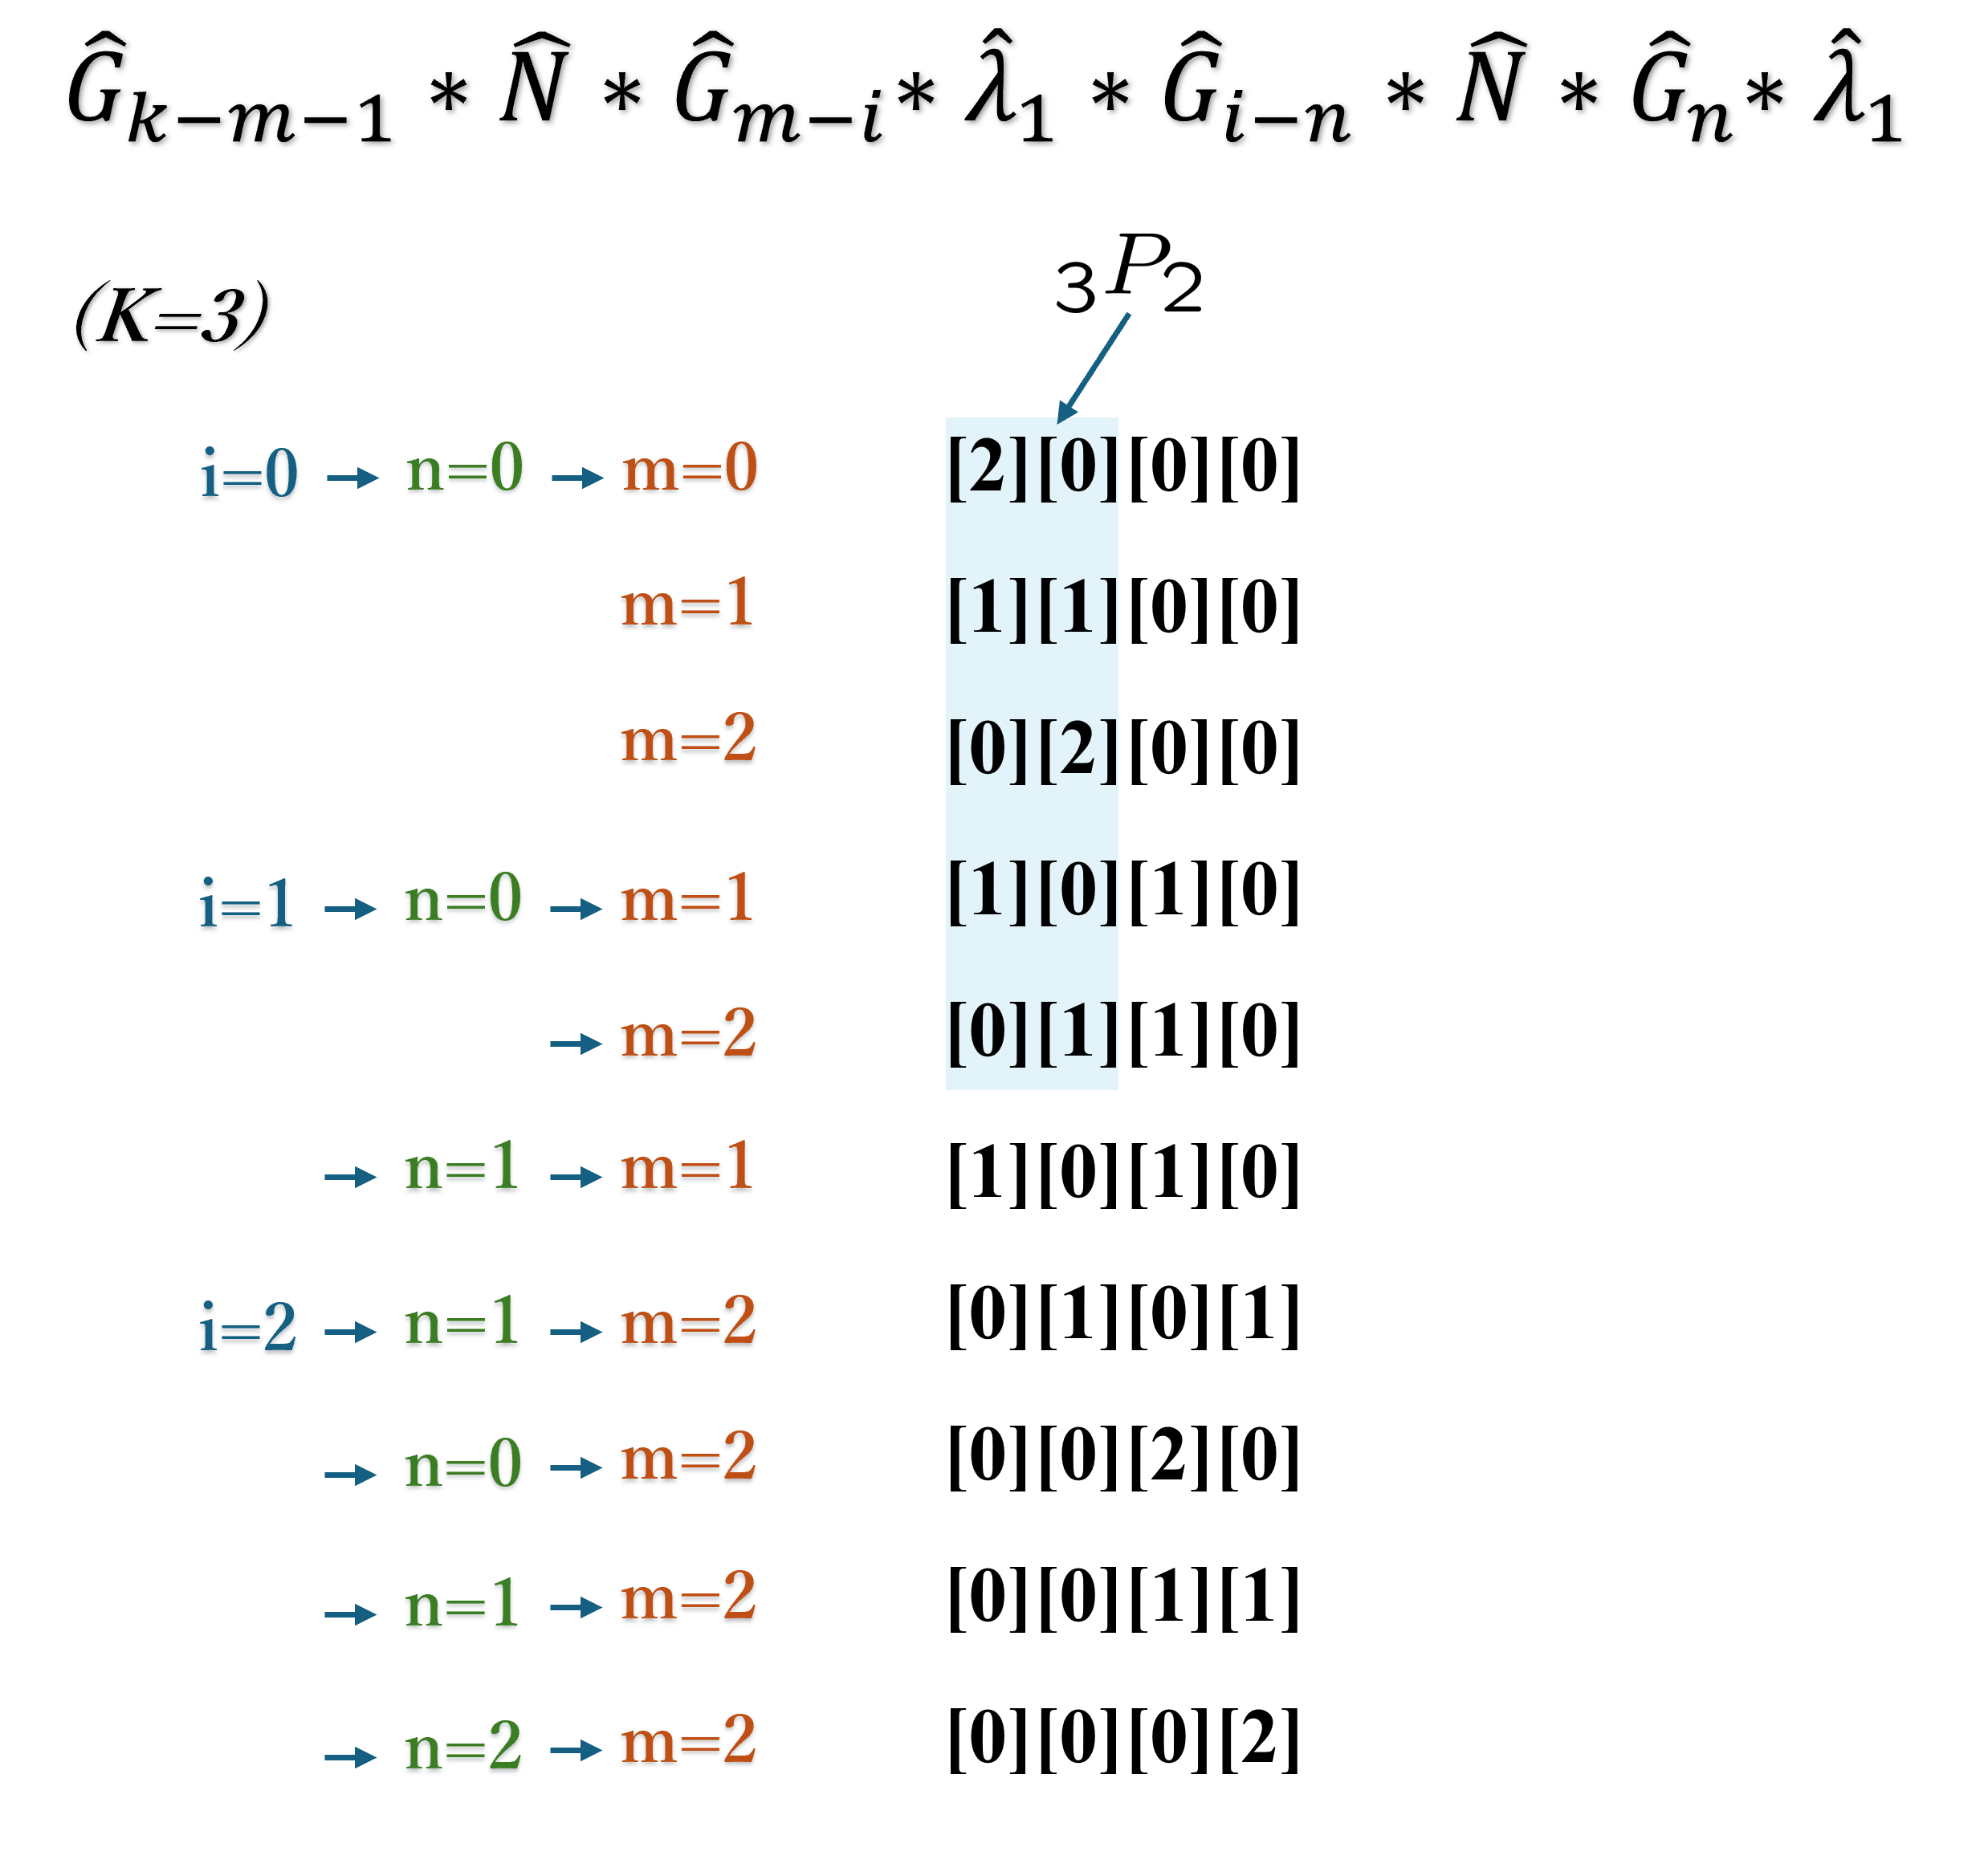
\includegraphics[width=12cm]{TexFigure/Tmat.png}}
  \caption{Possible calculation cases in k=3}
\end{figure}
Here, we can see that the total number of calculation cases can be represented by selecting and arranging two numbers from the three numbers 2, 1, and 0. To achieve this, we can introduce the following matrix:
\begin{figure}[htbp]
  \centerline{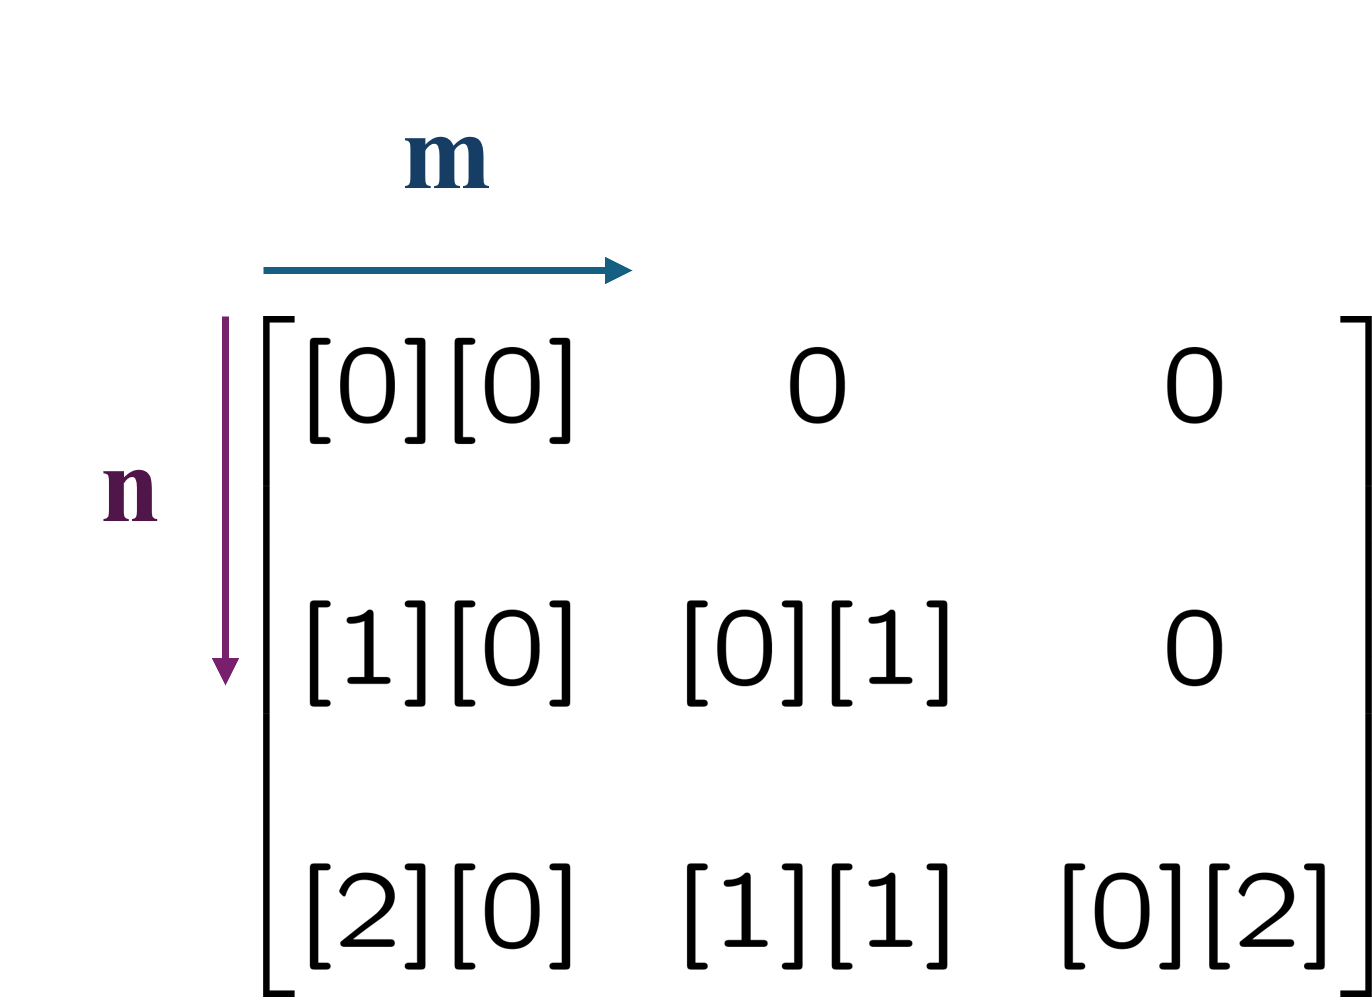
\includegraphics[width=9cm]{TexFigure/Tmat2.png}}
  \caption{The Structure of correlation-matrix}
\end{figure}
For example, if we want to represent all the possible cases as shown above, using the matrix above and calculating as below, we obtain all possible calculation cases.
\begin{figure}[htbp]
  \centerline{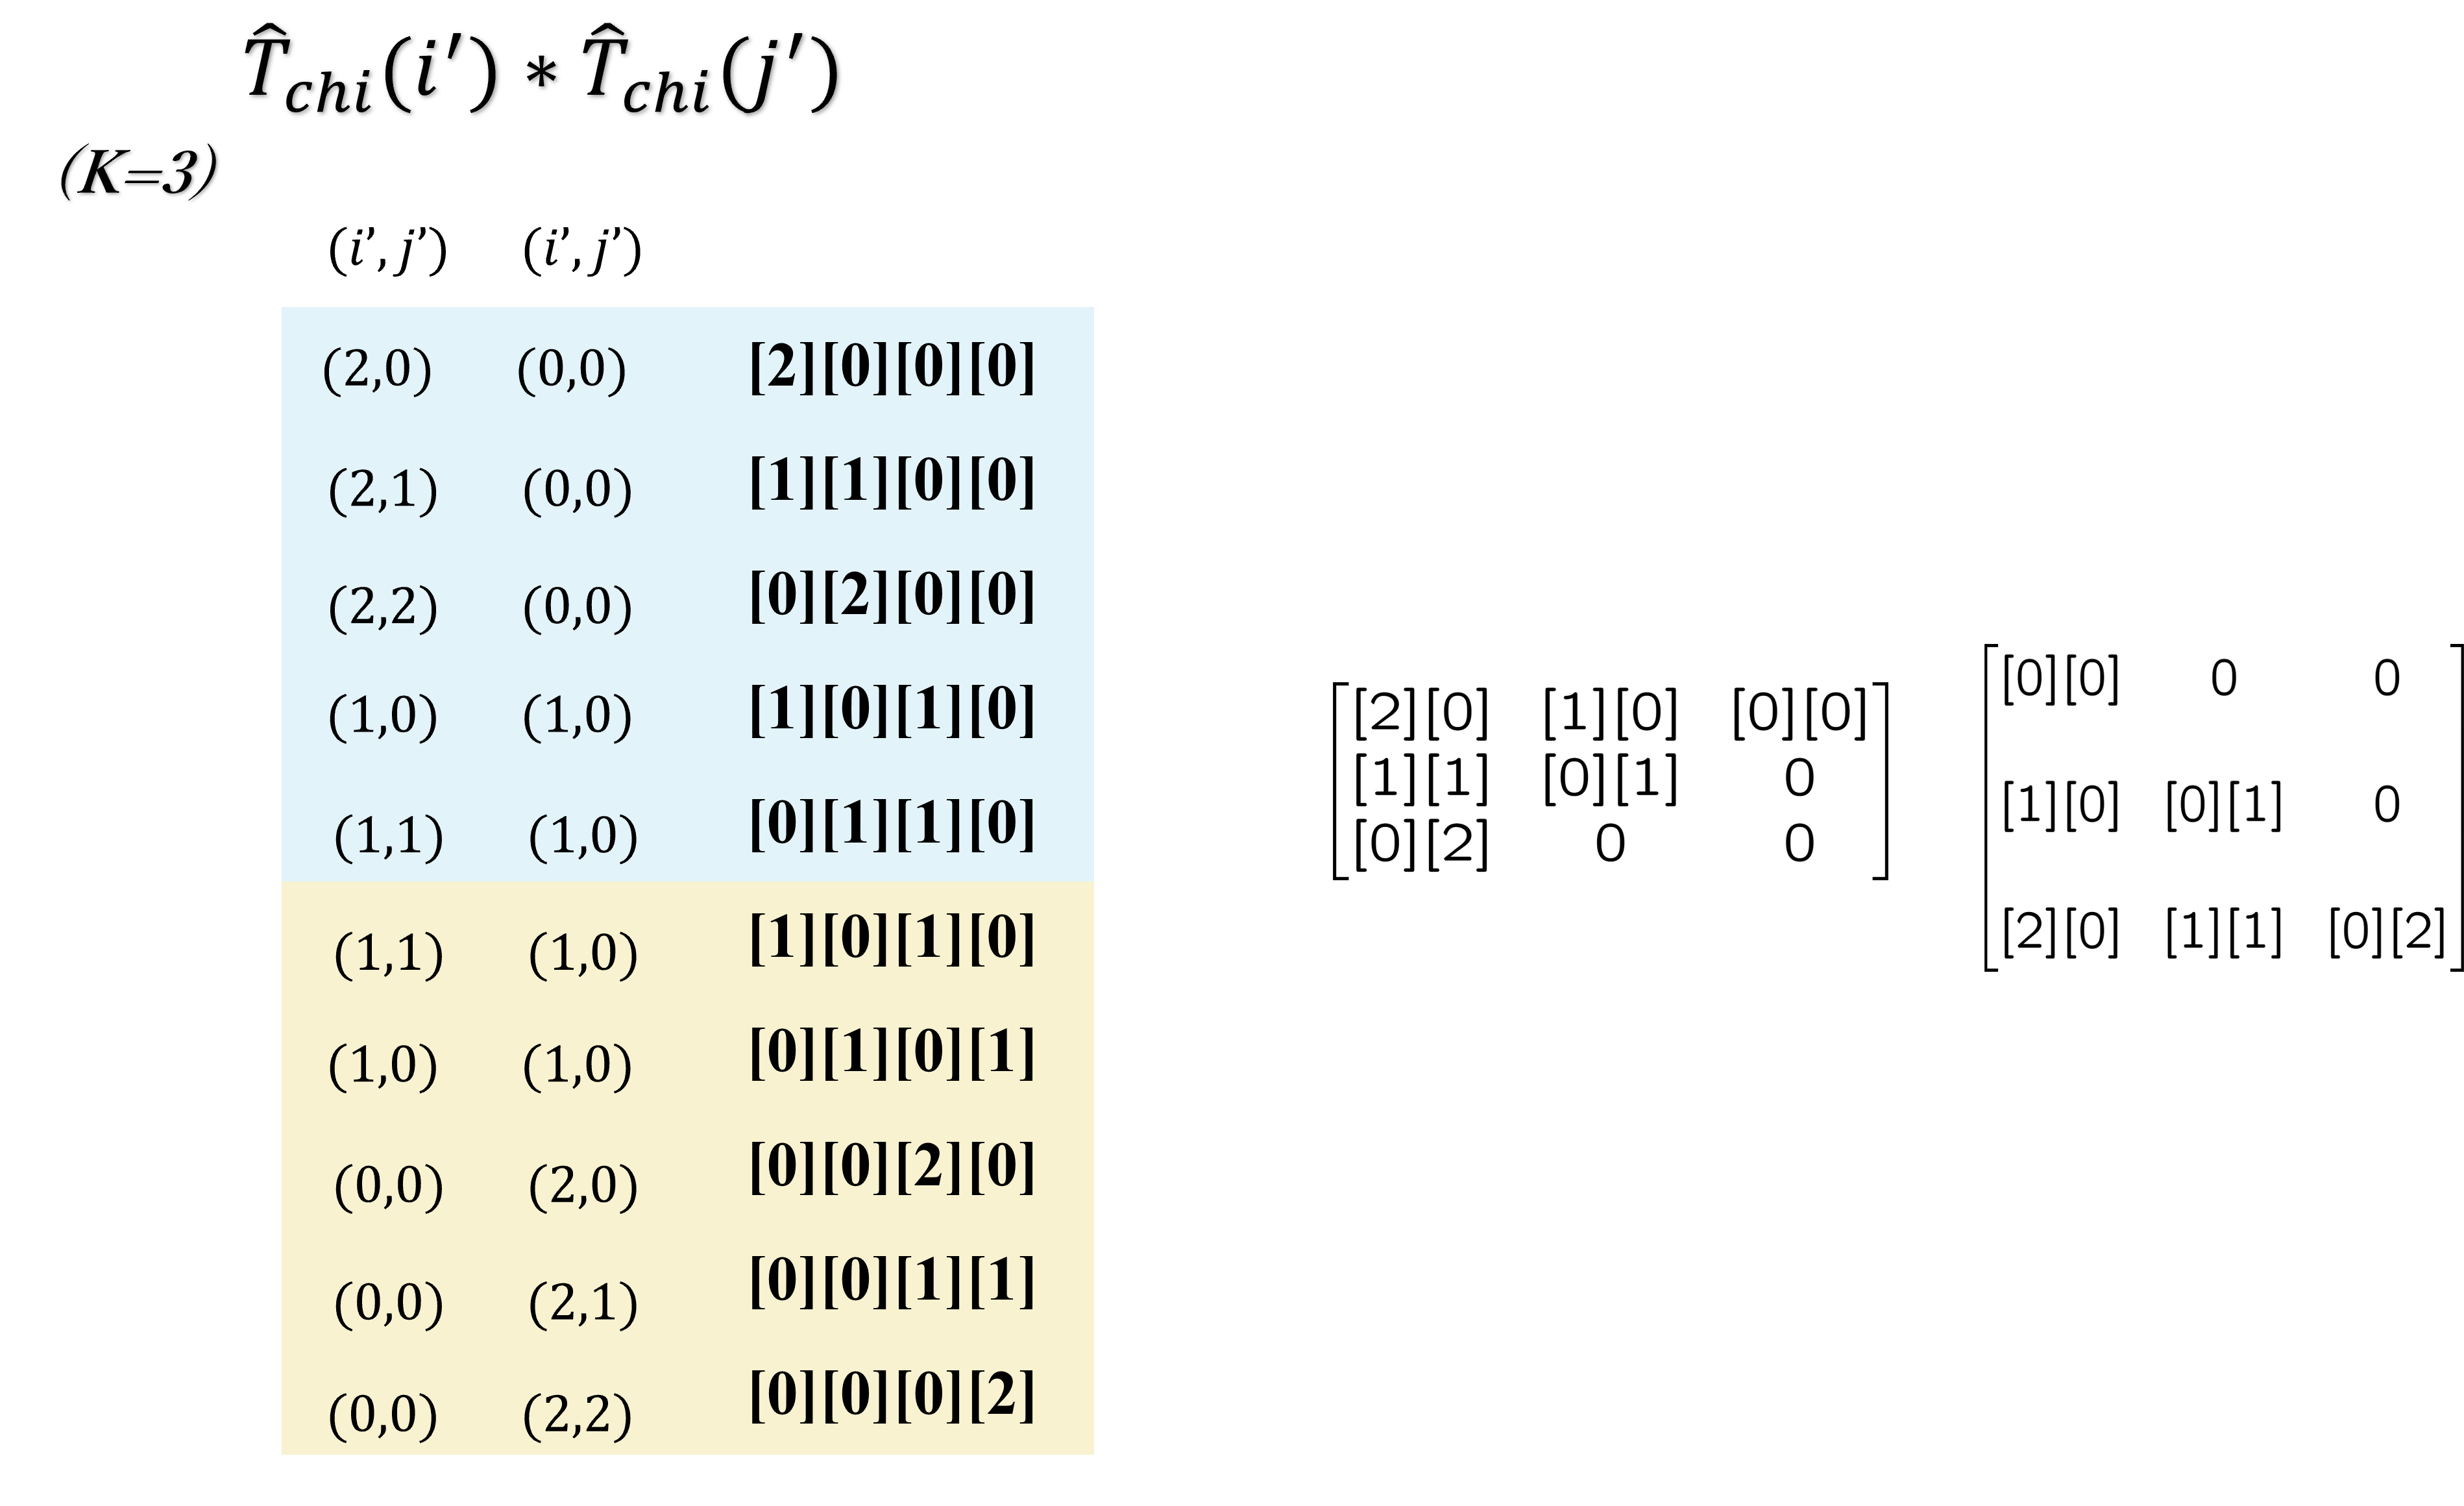
\includegraphics[width=12cm]{TexFigure/Tmat3.png}}
  \caption{Calculation using correlation-matrix}
\end{figure}

\pagebreak

\end{spacing}

\end{document}